\begin{savequote}[75mm] 
The Artificial Intelligence is the New Electricity.
\qauthor{Andrew Ng} 
\end{savequote}

\chapter{Principles of Machine Learning}
\label{chapter:ML}
This chapter provides a formal introduction to Machine Learning. It begins by presenting the concept of supervised learning. Next section is dedicated to discussing each of the models, which were taken into consideration during the author's research. It contains a brief mathematical description of each model and the overall approach to training them. The next section introduces the methodology of how the performance of each model can be measured and discusses the problem of the model's prediction interpretation. In other words, it tries to answer the vital question, "why should I trust the model that I built?". 
The final section covers the idea of bonsai Boosted Decision Trees, which are the binned version of this classifier. It explains the concept of discretization, its implementation, the reason this approach was chosen, and the issues it addresses. 

\section{What is Machine Learning?}
This introductory section is dedicated to providing answers to the following questions: 
\begin{itemize}
    \item What is Machine Learning? 
    \item Are there any difference between Machine Learning and classical algorithms? 
    \item What types of Machine Learning models can be distinguished? 
    \item Why is Machine Learning becoming more and more popular? 
    \item What kind of problems can Machine Learning solve? 
\end{itemize}

The classical approach to building software contains the following steps: collect system and software requirements,
design the software architecture, then there is a coding and testing part, and the software finally goes to the maintenance phase. The presented model is the simplest one called the Waterfall\footnote{The other approach to the software project management is called \textit{agile}, which is a practice that promotes continuous iteration of development and testing throughout the software development life-cycle of the project. Both development and testing activities are concurrent.}. The most important part is the coding phase, in which the developer or group of developers need to convert the system requirements, written in the Natural Language, into the code, which is understandable by a computer. They have to create a step-by-step set of instructions to process an individual input to determine the exact output. 
This strategy is not sufficient for many problems such as spam detection, image processing, or Natural Language understanding. For instance, the number of possible scenarios, e.g., sentences to translate from English to Polish, is so enormous that it is infeasible to create a dedicated logic for each of them. 

In such cases, Machine Learning comes to the rescue. Instead of writing explicit instructions, a researcher can provide examples and train the model using the data to extract the hidden patterns. The only remaining problem is to collect a sufficient amount of good quality data. However, is it a problem at all? 

Figure \ref{fig:big_data} shows the quantity of data generated per minute by the most frequently used online services. Facebook recently reported that the system that is designed to collect the logs generates about 2.5 PB of data per second \cite{facebook}, this is the approximate amount of the filtered data collected by the LHCb experiment during one year of nominal data taking. Another example of the online service that generates a massive amount of data is Twitter, according to its technical report, Twitter's users compose messages that required about 8 PB/day of data storage. One of the most challenging problems that the industry needs to solve is to understand the data and make a profitable conclusion based on it.

\begin{figure}[h]
\centering
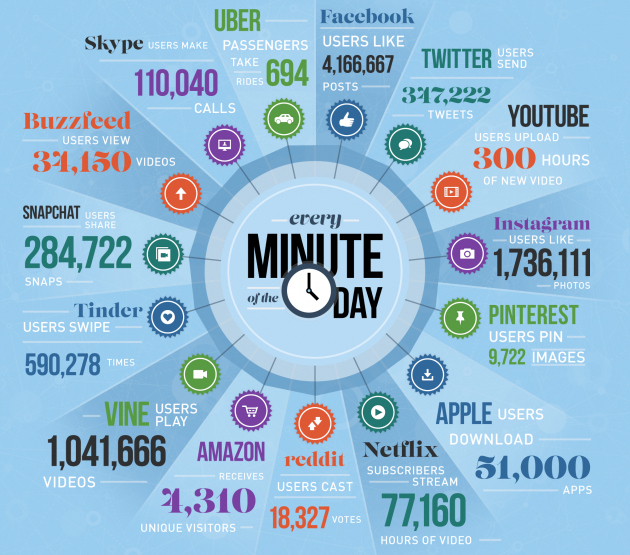
\includegraphics[scale=0.8]{figures/big_data.jpg}
\caption{The amount of data generated per minute by the most popular online services.
\label{fig:big_data}}
\end{figure}

Machine Learning as a discipline can be divided into three main areas: \textbf{supervised},\textbf{unsupervised} and \textbf{reinforcement learning}. Figure \ref{fig:ML_types} presents all mentioned types of Machine Learning approaches together with a description of problems that can be solved by them. 

The unsupervised learning describes problems, where the data has no manually assigned target value. One of the most interesting unsupervised problems is synthetical data generation. It is is usually performed using the idea of Generative Adversarial Networks (GANs) \cite{GAN}. Another type of unsupervised problem is a dimensionality reduction, which reduces the number of random variables under consideration by selecting a set of principal variables. 
One of the methods that are widely used to achieve this goal is the PCA or Principal Component Analysis. 
PCA is a statistical procedure that reduces the dimensionality of the dataset by creating new uncorrelated variables that successively maximize variance. Finding such new variables, called the principal components, reduces to solving an eigenvalue/eigenvector problem \cite{PCA}. 

Reinforcement learning employs an agent that interacts with an external environment and tries to learn the optimal behaviour strategy. This approach may lead to creating the program, that is capable to archive superhuman performance in such games as chess or Go \cite{alphago}, or can solve problem of protein folding \cite{alpha_fold}. The theory and application of the reinforcement learning is beyond the scope of this thesis, however author recommend the book \cite{suton_barto}, which the best resource to study this topic, and what is even more important it is available for free.     

\begin{figure}[h]
\centering
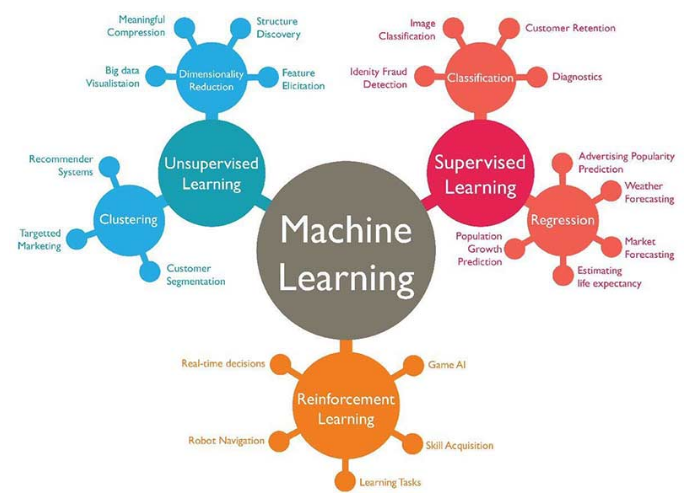
\includegraphics{figures/ML_types.png}
\caption{Graph showing the hierarchy of types of Machine Learning problems. 
\label{fig:ML_types}}
\end{figure}

Finally, supervised learning is a group of problems that are characterized by the presence of label that is assigned to each of the data examples. Supervised learning can be further split into classification and regressions tasks.
 Regression is a method of modelling a continuous target value (label) based on independent variables (predictors). This method is mostly used for forecasting \footnote{One of the examples that are usually used when the regression problem is introduced is finding a house price when such features as house area or the number of bedrooms are given.} and finding out the relationship between variables. 
 From the perspective of this thesis, the classification is the most important type of problem. Therefore the remainder of this section will focus on it.  In this task, the model tries to find the mapping between the input space and one of the \textit{k} labelled output. 
 
As a concrete example, let us consider a problem of a real track segment (or seed) selection, which is a topic of chapter~\ref{chapter:PLLT}. This is a supervised classification problem because the input to the model was a pair $(track_seed, label)$, which were obtained using Monte Carlo simulation, and the task is to predict whether a particular seed is suitable for further processing.

To give a more precise and formal definition of the classification task, let us consider a given set of $N$ training examples of the form \\ $\{(x_0,y_0), \dotsb , (x_{N-1} , y_{N-1})\}$, where $x_{i} \in R^{M}$ is a M-dimensional feature vector and $y_i \in \mathbb{N}_{>1}$\footnote{Within the context of this thesis, the one class classification problem, e.g. an outlier detection, is not not taken into consideration as a classification one} is a label. During the training phase, an algorithm tries to find the function $f: X\rightarrow Y$, where X is an input space and Y is the output space. The fitted function $f$ is an element of some space of all possible mapping functions, which by convention, is called hypothesis space and denoted as $\mathcal{H}$. To measure how well the function $f$ fits to the training data, a loss function $\mathcal{L}(y,f(x))$ needs to be defined \cite{DLBook}. This function reduces all the various good and bad aspects of a possibly complex system down to a single number. This scalar value allows candidate solutions to be ranked and compared to others.


When a loss function is selected the training procedure aims to minimize it with respect to the fitted function's parameters (these are the parameters of the selected model). This statement can be formalized in a following way: 
\begin{equation} \label{eq:loss}
f^*(x) = \underset{f \in \mathcal{H}}{\mathrm{argmin}} ~  \mathcal{L}(y,f(x))
\end{equation}
where $f^*(x)$ is an optimal, from the perspective of minimizing the loss function with respect to the training data, function belonging to $\mathcal{H}$, and $ \underset{x}{\mathrm{argmin}}$ is an operator when applied to a given function picks out the point in the function's domain at which its takes its minimum value (assuming that the point is unique), which can be formalized:
% buba
% ten kawałek dyskutowaliśmy i nie jest niestety poprawiony... dotyczy to też formuły
% zapisanej poniżej 
% buba

\begin{equation}
   \underset{\zeta \in S\subseteq \Zeta}{\operatorname{arg\,min}}\, \Phi(\zeta) := \{\zeta \mid \zeta \in S \wedge \forall \xi \in S : \Phi(\xi) > \Phi(\zeta)\}
\end{equation}
where $\Phi:\Zeta \rightarrow Y$, and the $S$ is a subset where the function $\Phi$ is defined.  

\paragraph{Information Theory} \mbox{}
 
To get a better understanding of a common choice for the cost function, the remainder of this section provides a brief introduction to the Information Theory.
Back in 1964, Claude Shannon and Warren Weaver published the paper "The mathematical theory of communication" \cite{Shannon}, where they introduced the concept of information entropy. This quantity was used to determine the optimal, with respect to the expected length,  message encoding. The basic intuition behind the entropy is that more likely events are less informative than the rare ones. To be more precise, the entropy needs to fulfil the following requirements:
\begin{enumerate}
\item Rare events should have high information content. 
\item In opposition, likely events should have very low information content, and in the case of a certain event, the information content should be $0$. 
\item The information content of two independent events should be equal to the sum of it. 
\end{enumerate}
To satisfy above properties, the Shannon entropy is defined in the following manner:  
\begin{equation}\label{eq:entropy}
H(P) =\mathbf{E}_{x\sim P}\left[\frac{1}{log P(x)} \right] = - \mathbf{E}_{x\sim P}[log P(x)] = - \sum_{i=1}^{n} P(x_i)log P(x_i)
\end{equation}
Where: $P(x)$ is the probability distribution of an event $x$ to occur, $\mathbf{E}$ is the expectation value operator, and $x \sim P$ signifies that random variable $x$ comes from distribution $P$. To summarize, the Shannon entropy measures the expected amount of information drawn from distribution $P$. It provides a lower bound on the length of encoding needed, on average, to encode a symbol taken from distribution $P$, which is visualized in figure \ref{fig:entropy}.
%buba - wydaje się, że zdanie powyższe jest przerwane w środku?
% fixed 

\begin{figure}[h]
\centering
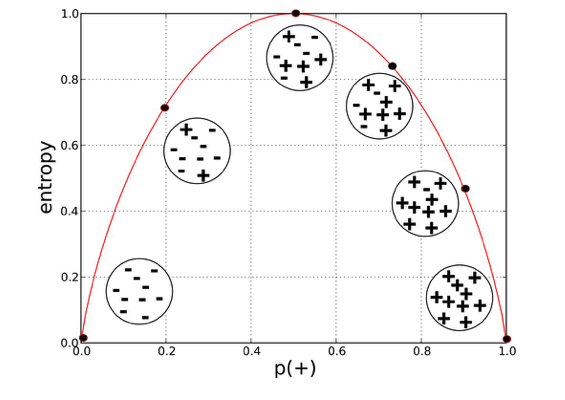
\includegraphics{figures/Entropy.png}
\caption{Visualization of the information entropy. The x-axis measures the proportion of data points belonging to the positive class, and the y-axis axis measures their respective entropies. Entropy is lowest at the extremes when the data either contains no positive instances or only positive instances. That is, when the data set is pure, the disorder is 0. Entropy is highest in the middle where the data is evenly split between positive and negative instances. Extreme disorder, because there is no majority. Figure adapted from \cite{DS_for_buisness}   
\label{fig:entropy}}
\end{figure}

As an example, let us consider a variable $m$ that has four possible states \\ $(a, b, c, d)$ for which the respective probabilities are given by \\ $(\frac{1}{2},\frac{1}{4},\frac{1}{8},\frac{1}{8})$.
The naive approach, where the creator of the encoding does not leverage the information about respective state probabilities, would require to transmit a message of length 2 bits. Although, taking into consideration the nonuniform probability of each state, the entropy can be expressed in the following manner: 

\begin{equation}
    H(m) = \frac{1}{2} log(\frac{1}{2}) + \frac{1}{4}  log(\frac{1}{4}) + 2 \frac{1}{8} log(\frac{1}{8}) =1.75
\end{equation}
Which indicates that providing a better encoding the sender can save, on average, 0.25 bit per message. The example, encoding that gives a shorter code to the more likely events, using for instance the following encoding $\{a:0, b:10, c:110, d:111, \}$. For such a encoding the average message length is equal to: 
\begin{equation}
\label{eq:entropy example}
    \text{average code length}= \frac{1}{2}\cdot 1 + \frac{1}{4}\cdot 2 + \frac{1}{8}\cdot 3 = 1.75 \text{bits}
\end{equation}

Equation \ref{eq:entropy example} shows a very interesting relation between entropy and optimal coding. In general, the entropy is a lower bound on the number of bits needed to transmit the state of a random variable. There is no way to get an average message length smaller than the entropy value.   

The concept of entropy can be extended to the case of two separate probability distributions $P(x)$ and $Q(x)$ over the same random variable $x$.  In such a case, the quantity called \textbf{Cross Entropy}  measures the amount of information needed to send a message containing symbols drawn from distribution $P(x)$, when using encoding designed to minimize the length of messages coming from the probability distribution $Q(x)$.  
The cross-entropy is defined in a following way:

\begin{equation}
H(P,Q) = - \mathbf{E}_{x\sim P}[log Q(x)] = - \sum_{i=1}^{n} P(x_i)log Q(x_i)
\end{equation}
One of the key properties of the cross-entropy is the fact that it is always non-negative. It shall take the minimum value of $0$ only when $P(x)$ and $Q(x)$ are the same distributions. Therefore, the cross-entropy can be interpreted as kind of a distance metric, that measure similarity between two distributions. For the binary classification, this is the case where the number of classes to predict $k=2$, the cross-entropy simplifies into the following form:

\begin{equation}
\label{eq:CE_binary}
   \mathcal{L} = -y \ln\left( f(x) \right) - (1-y) \ln\left(1 -f(x) \right)
\end{equation}


Figure \ref{fig:ML_flow} presents a typical methodology to build a Machine Learning system in the form of a flowchart. 
Within this process, we can distinguish two phases: Creation and Production. The creation phase starts by collecting the data, and then the entire data is split into two subsets of training and testing samples. The former is usually divided into two disjoint sets training and validation sets.

The training set is used to select the hypothesis function, and the test set is used to verify the model's performance.
The process of training the model is usually a very complicated iterative procedure, which consists of such steps as selecting the hypothesis space, finding an optimal set of model's hyperparameters, etc. The way to robustly and properly measure the goodness of the model fitting is very often based on metrics calculated using cross-entropy.

\begin{figure}
\centering
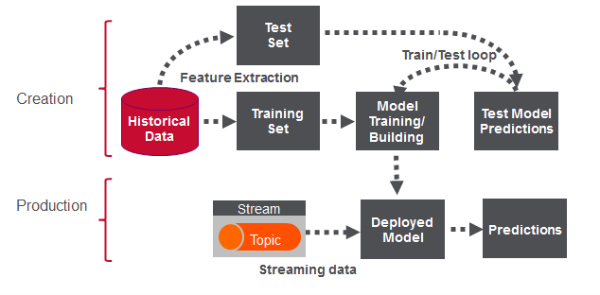
\includegraphics{figures/MLflowchart.jpg}
\caption{Simplified Machine Learning flowchart
\label{fig:ML_flow}}
\end{figure}


\section{Classification metrics overview}
\subsubsection{Confusion matrix}
The starting point in every discussion of the classifier performance measurement is a confusion matrix. Karl Pearson invented the idea of the confusion matrix in 1904. For a binary classification problem, the outcome of the classification can have four possible values. If the particular example has a positive label \footnote{In the field of High Energy Physics the positive example is usually called the signal, and the negative one the background} and the classification result is positive the outcome is called \textbf{true positive}; if it is classified as negative, it is counted as \textbf{false negative}. In case the true label was negative, and the classification estimated negative, it is counted as \textbf{true-negative}. Otherwise, the outcome is called \textbf{false-positive}. The false-positive and false-negative are also known as, using statistical language, type I and type II error, respectively. 
A two-by-two matrix can be constructed for better understanding and visualization of the classification outcome using the set of examples, usually called the test set. Figure \ref{fig:CM} shows a confusion matrix along with equations of selected standard metrics that can be derived from it. The elements from the diagonal represent the correct decision made by the classifier. In opposition, the off-diagonal numbers correspond to the miss-classified examples. 

\begin{figure}[h]
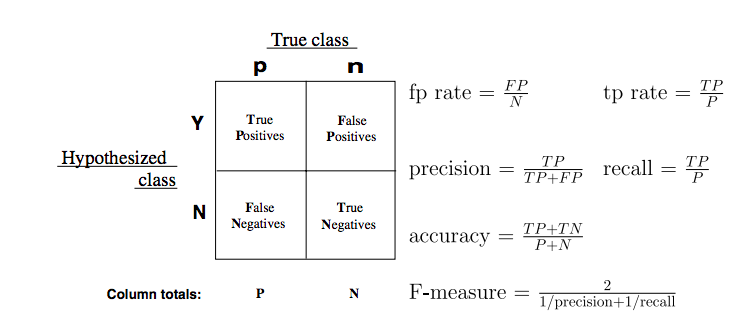
\includegraphics[width=\textwidth]{figures/ConfusionMatrix.png}
\caption{Confusion matrix and common performance metrics derived from it along with their respective formulas. 
\label{fig:CM}}
\end{figure}

Using the information that the Confusion Matrix is built on, one can calculate the following quality metrics:

\begin{itemize}
    \item $\mathbf{accuracy} = \frac{TP+TN}{P+N}$, defines the number of examples that were correctly classified. Note, this quantity may be misleading. Consider the problem of an imbalanced dataset where the number of positive examples is 98\% of the entire dataset. The dummy classifier, which always returns 1, achieves a 98\% accuracy score.
    \item $\mathbf{precission}=\frac{TP}{TP+FP}$; measure what proportion of events, that were correctly classified as a given class to all events that were classified as this class. Precision is a good measure to determine when the costs of False Positive is high. 
    \item $\mathbf{recall}=\frac{TP}{TP+FN}$ actually expresses how many of the actual positives model correctly classified. Recall shall be the model metric in use to select the best model when there is a high cost associated with False Negative. Recall can be interpreted as a measure of the model's sensitivity.
    \item $\mathbf{F1} =\frac{2}{\frac{1}{precision}+ \frac{1}{recall}}$ should be use, when one seeks for a balance between Precision and Recall and there is an uneven class distribution. 
\end{itemize}

\subsubsection{Receiver operating characteristics}
\label{sec:ROC}
The Receiver Operating Characteristics graphs are two-dimensional plots where the true positive
rate (Y-axis) is plotted against the false positive rate (X-axis). A ROC graph depicts relative trade-off between benefits (true positives) and costs (false positives).  

Figure \ref{fig:ROC_eg} presents a sample of a ROC graph comparing different discrete classifiers. That kind of classifiers for a given input sample returns a single number as a decision, in the case of binary classification it is Yes or No decision. The origin, point (0,0), represents the classifier, which never issuing a positive classification outcome, which means its prediction regardless of the input vector is always 0. Such a classifier commits no false-positive errors but also gains no true positives. On the contrary, point (1,1) represents classifier, which always returns a true value. Generally, all points that lay on a straight line that satisfies equation $y=x$ correspond to the random guessing policy, and the corresponding classifiers are useless, and they have not extracted any patterns from the data.  

Point D $(0,1)$ corresponds to the perfect classification, which means all negative examples are suppressed, and all positive are preserved. In general, the classifier is better than another if its corresponding point in a ROC space is to the northwest\footnote{oriented according to the compass rose} of the first. 
% buba
% zrób odnośnik do rysunku 3.2.2 i w podpisie zdefiniuj co to jest west a co to jest north
% opis poniżej trzeba zdecydowanie odnieść do rysunku 
% 
% Huh, that was challenging. How to define NSWE directions? Sometimes the easiest things are the hardest to define (like time)

Classifiers appearing on the upper right-hand side of a ROC graph may be considered as a \textit{liberal}. They make positive classifications with weak evidence, so they classify nearly all positives correctly, but they often have high false-positive rates. Therefore the point A is more conservative than point B. The point E corresponds to the strategy, which is worst than the random guessing; this indicates some issue with data labelling, Usually, there are no such points in practical applications. 

\begin{figure}[!ht]
\centering
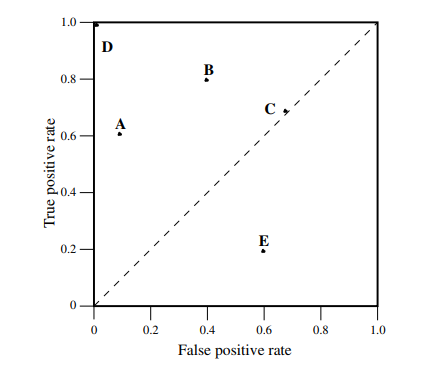
\includegraphics[scale=0.7]{figures/ExampleROC.PNG}
\caption{A exemplary Receiver Operating Characteristics graph indicating the performance of five discrete classifiers.
% buba zdefiniuj kierunki
% already defined in the footnote 
\label{fig:ROC_eg}}
\end{figure}

Most of the classifiers, instead of returning a discrete value, return a probability measure also called the score. These probabilities can be compared to thresholds to produce the binary classification.  Each threshold value produces a different point in the ROC space, and a collection of those points creates the ROC curve. The ROC curve is a very convenient way to find a classifier's operating point. 
The curve provides a convenient diagnostic tool to investigate one classifier with different threshold values and the effect on the True Positive Rate and False Positive Rate. One might choose a threshold in order to bias the predictive behaviour of a classification model. For instance, in the case of the track seed classification problem, the classifier has to preserve almost all true tracks while keeping the background as low as possible. Therefore, the classification threshold should be selected so that the true positive rate would be equal to 0.99.  

ROC curve is a popular diagnostic tool for classifiers on balanced and imbalanced binary prediction problems alike because it is not biased to the majority or minority class. ROC analysis, in opposition to the study based on accuracy metrics, does not have any bias toward models that perform well on the majority class at the expense of the minority one, which is a desirable property that is quite attractive when dealing with imbalanced data \cite{imbalanced_learnig}.

The ROC curve is a two-dimensional representation of classifier performance. This representation may not be convenient when comparing the performance of two or more classifiers.  
 Thus, it is customary to reduce the ROC curve to a single scalar value representing the expected classifier performance while keeping its properties. The common practice is to calculate the Area Under the ROC Curve (ROC AUC).  From the statistical point of view, the ROC AUC can be interpreted as a probability that the classifier will rank a randomly chosen positive example higher than a randomly chosen negative sample. 

\section{Model selection}

This section provides a detailed description of the model selection and validation procedure. Within the scope of this project, four different models were tested. Each of the subsection starts by presenting the mathematical formalism of a particular model. The next part focuses on applied methodology to find the optimal, in the sense of maximizing the selected metric score, set of model's hyperparameters, see section \ref{sec:hyperparameters}. 
The first two presented models were constructed using the sklearn \cite{sklearn} and the numpy \cite{numpy} libraries. 
% buba - odnośnik poproszę...
% I wated to add references to the numpy paper (Nature). Highly recommend to read it. 

\subsection{$k$-Nearest Neighbors classifier}
\label{sec:knn}
The $k$-NN was selected to play the role of a study baseline. The $k$-NN  is a \textbf{non-parametric} model, which means it takes no assumption on the underlying probability distribution of data \cite{knn}. 
Instead, the model's fundamental assumption is that similar inputs should produce similar outputs. To make a prediction, the model looks at the K points in the training set nearest to the input $x_i$ and counts how many members of each class are in this set and finally returns the empirical fraction as the estimate. That statement can be formalized in terms of probability:  

\begin{equation}
p(y=k,\mathcal{D}, K) = \frac{1}{K} \sum_{i\in N_K(x,\mathcal{D})} \mathds{1}(y_i=k)
\end{equation}
where: 
$N_K(x,\mathcal{D})$ are the K nearest points to x in $\mathcal{D}$ and $\mathds{1}(y_i=k)$ is the indicator function defined as follow: 

\begin{equation}
    \mathds{1}(e) = \left\{ \begin{array}{ll}
1 & \textrm{when e is true}\\
0 & \textrm{when e is false}\\
\end{array} \right.
\end{equation}

In order to make a prediction, the algorithm needs to evaluate the following steps: 
\begin{algorithm}[caption={k-nearest neighbour, $k$-NN }, label={knn}]
Data: Training data ${x^{train}_{i} , y_{i}}$, and test data ${x^{test}}$
Result: Predicted test output $\hat{y}$
Load the training and test data;

Find the k training data points $x_i$, which has the shortest distance$\mathcal{D}(x^{train}_i, x^{test})$;
Decide $\hat{y}$ with a majority vote among those k nearest neighbours;  
\end{algorithm}

The number of neighbours $k$ and distance function are the only two hyperparameters that need to be selected apriori by a Machine Learning practitioner. In the case where the choice is not intuitive, usually, an extensive scan of the parameter space should be performed as a part of the verification studies. Figure \ref{fig:knn decision boundary} visualize the influence of the different values of $k$ on the classifier decision boundaries. The decision boundary is a disjoint region where each of the points is classified into the same class. It is clearly visible that considering more neighbours produce a smoother decision boundary. 

\begin{figure}[!h]
   \centering
   \subfloat{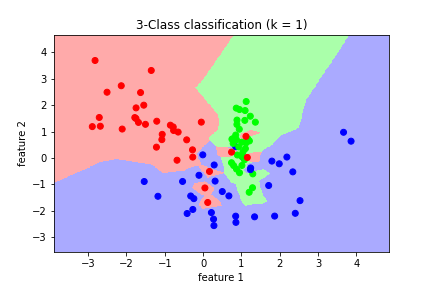
\includegraphics[width=.4\textwidth]{figures/KNN_1.png}}\quad
   \subfloat{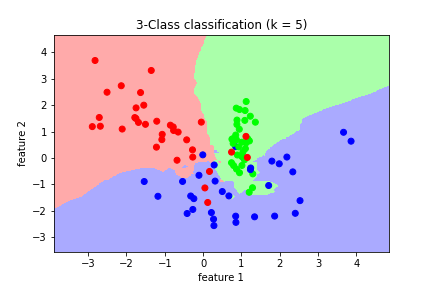
\includegraphics[width=.4\textwidth]{figures/KNN_5.png}}\\
   \subfloat{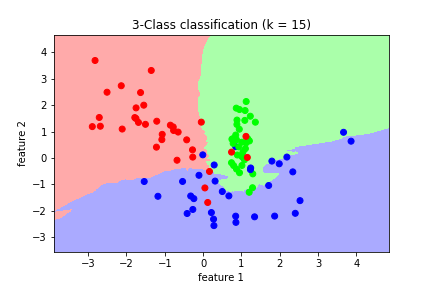
\includegraphics[width=.4\textwidth]{figures/KNN_15.png}}\quad
   \subfloat{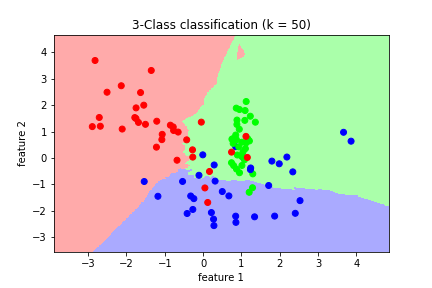
\includegraphics[width=.4\textwidth]{figures/KNN_50.png}}
   \caption{$k$-NN decision boundaries. Each plot was generated for a different value of the nearest neighbours. The data (100 points) and the labeling function used to generate these plots were selected randomly.
   \label{fig:knn decision boundary}}
\end{figure}

K-NN model has two limitations. First of all the K-NN's prediction time and space grow linearly with the number of training examples\footnote{There are a couple of methods like KD-trees that reduce K-NN evaluation complexity. Still, it does not affect the space complexity of the model}, which make this model infeasible when the amount of the data samples are very large (i.e., $10^{5} - 10^{6}$ events). The second limitation of the $k$-NN models is the fact that this model suffers from the\textbf{ curse of dimensionality}.  In low dimensional spaces, data may seem very similar, but the higher the dimension, the further these data points may seem to be. To illustrate this phenomenon let consider a collection of points $x_i$ that are sampled uniformly within the unit  $d$ dimensional hypercube $\forall i, x_i \in [0,1]^{d} $, and the model that is looking for $k=10$ neighbours of a particular test point. Let $l$ be the edge of the smaller hypercube that contains all $k$-nearest neighbour of a given test point, then 

\begin{align}
l^{d} \approx \frac{k}{n} \nonumber \\
l \approx (\frac{k}{n})^{\frac{1}{d}}
\end{align}

If the training dataset contains $n=1000$ entries each of dimensionality $d=20$, then $l \approx 80\%$, which means almost the entire space is needed to find the 10-NN. This breaks the $k$-NN  assumption because the $k$ neighbors are not particularly close to each other, and therefore similar, to any other data points in the training set. 
If we take into consideration that dimensionality of the track classification problem, it is not expected to get promising results. Although training the $k$-NN is pretty fast, so seems to be a reasonable choice for a baseline model. 

\subsection{Logistic Regression}
\label{sec:LogReg}
Another family of models that is usually trained in order to get a study baseline is Logistic Regression, which is one of the simplest parametric classification models. The name of this model may be confusing. Despite having term "regression" inside its name, it is a classification model. It is based on the assumption that the output is a linear function of the inputs: 
\begin{equation}
\label{eq:logreg}
    y(x) = \sigma (w^{T}x + b) = \sigma \left(\sum_{i=1}^{D}w_ix_i +b\right) 
\end{equation}
where: $w^{T}x$ is a dot product between the input vector $x$ and the model's weights $w$, and $b$ is a bias term. In this context, the bias term means the model's output when no input signal is given. Do not confuse with the statistical "bias", which represents the difference between true parameter value and the estimator's expected value. The $\sigma$ is a \textbf{sigmoid} function. It is defined as: 
\begin{equation}
\label{eg:sigmoid}
    \sigma(x) = \frac{1}{1+\exp(-x)}
\end{equation}
The term "sigmoid" means S-shaped, which is shown in figure \ref{fig:sigmoid}. This function is used to map the whole real axis into a finite interval. In the case of classification, it squashes the regression output (term $w^{T}x$) into the interval $\{0,1\}$, which can be interpreted as a probability. Positive input numbers become high probabilities, and the negative values become low ones. 
The first derivative of this function can be expressed in the following way:

\begin{equation}
    \frac{d\sigma(x)}{dx} = \sigma(x)\cdot(1-\sigma(x))
\end{equation}


\begin{figure}[h]
\centering
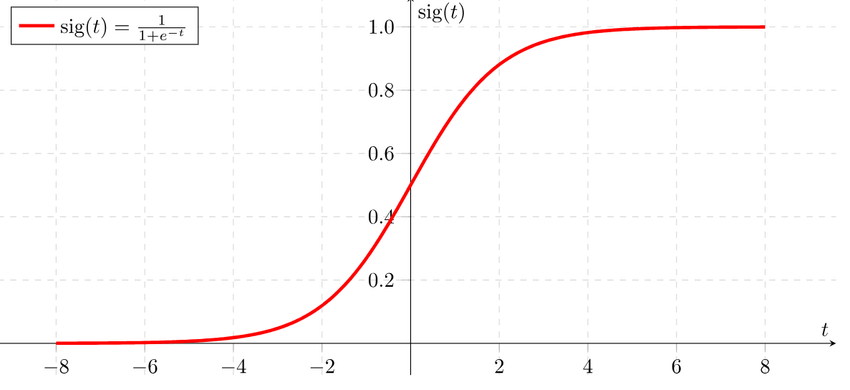
\includegraphics[width=\textwidth]{figures/sigmoid.png}
\caption{Plot of the sigmoid function.
\label{fig:sigmoid}}
\end{figure}

In the case of binary classification, $y \in \{0,1\}$, the model \ref{eq:logreg} can be rewritten in the following probabilistic form:

\begin{equation}
p(y|x,w) = B(y|\sigma(w^{T}x + b))
\end{equation}

where: $B(z|\theta)$ is a Bernoulli  distribution defined as:

\begin{equation}
    B(z|\theta) =  \left\{ \begin{array}{ll}
\theta & \textrm{if z = 1}\\
1-\theta & \textrm{if z = 0}\\
\end{array} \right.
\end{equation}
the $\theta$ is a probability of a success. The Bernoulli distribution is a special case of a binomial distribution, where $n=1$. 

The model fitting procedure
%\footnote{model fitting is an algorithm that aims to estimate the model's parameter using the data } 
can be derived using Maximum Likelihood Estimation (MLE) technique \footnote{ MLE is used to find $\Tilde{\theta} = \underset{\theta}{\mathrm{argmin}} log p(D|\theta)$, where $D$ is a data} \cite{bishop}. The likelihood function is a quantity similar in its nature to the probability. The difference is that the probability is used to describe the future outcome of the random process, and the likelihood tells what is the probability that observed data were sampled from the process described by some specific model and is a function of the model's parameters. 

For a dataset $D:=\{x_{n}, y_n\}$ where $y_{n} \in \{0,1\}$ and $n=1 \cdots N$ the likelihood of the entire dataset can be written as: 

\begin{align}
\label{eq:liklehood}
        L(w) &= \prod_{i=1}^{N} B(y_i|x_i, w) \nonumber \\
        &= \prod_{i=1}^{N} \sigma(w^{T}x_i)^{y_i}\cdot \left[1- \sigma(w^{T}x_i) \right]^{1-y_i}
\end{align}

The equation \ref{eq:liklehood} assumes that the training examples are independent and identically distributed (iid). In the practical application instead of maximizing the likelihood \ref{eq:liklehood} it is more convenient to minimize negative logarithm of likelihood according to the following formula:

\begin{equation}
\label{eq:NLL logistic}
    NLL(w) = \sum_{i=1}^{N}y_{i}log\left( \sigma(w^{T}x_{i}\right)+(1-y_i)log(1-\sigma(w^{T}x_{i}))
\end{equation}

Formula \ref{eq:NLL logistic} is identical to the cross-entropy \ref{eq:CE_binary} for a case when number of classes is two. This provides an additional justification for using cross-entropy as a cost function. 

The conventional approach to finding a minimum of the cost function and setting the derivatives of this function with respect to the parameters $w$ fails due to the lack of closed-form for the minimum. Instead, the iterative optimization algorithm has to be applied. Within the scope of this thesis, the Gradient Descent algorithm will be discussed.    

\paragraph{Gradient Descent Optimization} \mbox{}

The Gradient Descent is an optimization algorithm that attempts to find a minimum of a function by taking small steps in the direction of the gradient vector and ends at the local minimum. In the case of a linear model, it can be proved that it will always be a global minimum \cite{bishop}. The proof is based on analysis of the Hessian matrix, which for the case of linear model \footnote{Linear term in a linear model refers to the parameters but not necessarily to the features, for instance, $f(x)=w_1x+w_2x^2 + w_3 \sin(x)$ is considered as a linear model} is always positive defined\footnote{$n \times n$ matrix $M$ is positive defined if for all vector $\vec{x} \in R^{n}$ $\vec{x}^{T}M\vec{x} > 0$. Intuitively, a positive defined matrix is a matrix generalization of a positive number, which does not change the sign of the number}. 
That kind of optimization is called convex, and it is the reason why generalized linear models still play an important role in classical Machine Learning.  
During a single optimization step the new, updated value of the parameter $w_i$ is calculated according to the following formula: 

\begin{align}
\label{eq:Gradient decent}
    w_{i}^{new} &= w_{i}^{old} - \eta \cdot \frac{\partial \mathcal{L}}{\partial w_{i}^{old}} \nonumber \\
    &= w_{i}^{old} - \eta  \cdot \sum_{j=0}^{N} \left( \sigma((w^{old})^{T}x_{j}) - y_{j} \right) x_j
\end{align}
where: $\eta$ is a step size, also called learning rate, which has to be set before the training procedure and $\mathcal{L}$ denotes the loss function. The wrong choice of the learning rate value can pose a number of problem for the training algorithm, which is shown in figure \ref{fig:Gradient decent}. Setting it to a value that is too low may lead to a very long training process that may not be practical. On the other hand, setting too high may lead, in turn, to rapid oscillations in the loss function and usually, the algorithm will fail.

\begin{figure}[!h]
\centering
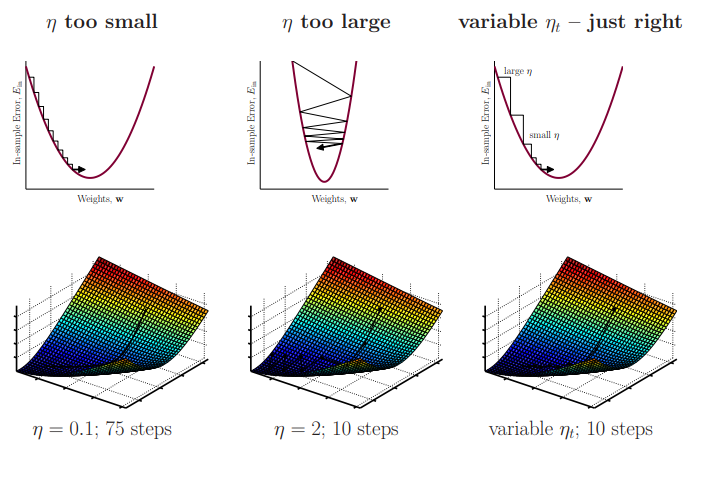
\includegraphics{figures/LR_learning_rate.PNG}
\caption{Comparison of the learning rate values and its influence on a final model performance. Figure taken from \cite{abu-musafa}  
\label{fig:Gradient decent}}
\end{figure}
The second parameter of the gradient descent algorithm \ref{eq:Gradient decent} is a number of examples $N$, that are used to calculate the new weights. There are three versions of this optimization method. The first one also called Stochastic Gradient Descent (SGD), update weights after each training example, which is equivalent to set $N=1$. For $N>1$ it is called Mini-batch Gradient Descent. The final method uses $N$ equal to all examples, and it is usually called Batch Gradient Descent. Those tree methods and the corresponding weight updates are visualized in figure~\ref{fig:Batch gradient decent}. The SGD frequently updates the model, which provides immediate insight into its performance and improvement rate. However, this method's downside is noisy gradient information, which may affect the model parameters to oscillate around the minimum value, which may reveal a higher variance over training epochs. On the other hands, the Batch version of the Gradient Descent require a lot of memory and can be very slow for large datasets, and more stable error gradient may result in coverage to less optimal local minimum.

%buba jak już wspominasz of paczkowaniu danych, to może wyjaśnimy dlaczego 
% paczkowanie może prowadzić do lepszych wyników?
% AD:  czy to wystarczy? Czy mam jeszcze dalej opisywac? 

\begin{figure}[!h]
\centering
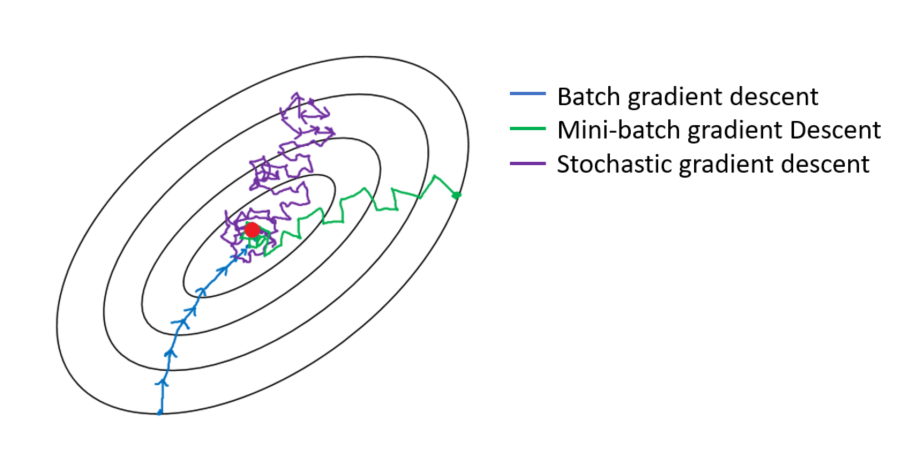
\includegraphics{figures/batch_descent.png}
\caption{Comparison of the different variants of the gradient descent algorithms and its influence on weights update path toward minimum.
\label{fig:Batch gradient decent}}
\end{figure}


Several enhanced versions of GD algorithm were proposed in the literature, the summary of them can be found in \cite{GradientDescent}. 
From the perspective of deep learning, which is a topic of section \ref{sec:DNN}, the ADAM optimization algorithm is the most recommended one \cite{ADAM}. 

\paragraph{Regularization} \mbox{}
\label{sec:regularization}
When training any classification model, the general task is to make it perform well not only on a training set but also on a new, previously unseen data sample. This objective is called generalization and can be quantified by a test error. One of the strategies to reduce the gap between training and test errors is called regularization. There are many forms of regularization. Within this thesis's scope, the modification of the cost function \footnote{The other popular regularization method is data augmentation, which is used to generate a new training example by applying some transformation function on old examples. The proper choice of a transformation function in the case of high-dimensional tabular data is not obvious; that why it was not implemented.} in order to discourage the parameters from reaching a large value. A model with one or a few large parameters means that model is using only a small subset of features to make a decision. To avoid that kind of situation, the additional penalty term can be added to the loss function: 

\begin{equation}
    \mathcal{L}_{reg}(w) = \mathcal{L}(w) + \Omega(w) 
\end{equation}
where: $\mathcal{L}$ is the previous, non-regularized loss function, and the $\Omega(w)$ is a regularization term that is a function of a model's weights. 

The simplest and most popular choice of the $\Omega(w)$ is a sum of squares of the the model's coefficients\footnote{that kind of regularization is also called Ridge Regression or $L^2$}. In such a case, the cross-entropy loss function \ref{eq:CE_binary} is expressed by the following formula:

\begin{equation}
    \mathcal{L} =  \sum_{i=1}^{N}y_{i}log\left( \sigma(w^{T}x_{i}\right)+(1-y_i)log(1-\sigma(w^{T}x_{i})) + \frac{\alpha}{2} w^{T}w
\end{equation}
where: $\alpha$ is a hyperparameter that weight a relative contribution of a squared norm penalty. 
That kind of regularization is also known as weight decay. It can be shown  that the addition of the $L^2$  regularization term modifies the learning rule to shrink the weight vector on each optimization step. 

The second popular way of expressing $\Omega(w)$ is called a lasso regression:
\begin{equation}
\label{eq:lasso}
    \Omega_{l_1}(w) = \frac{\alpha}{2} ||w|| = \frac{\alpha}{2} \sum_{i=1}^{M} |w_i|
\end{equation}

 Adding the lasso regularization term is equivalent to a feature selection mechanism. The proof of this statement is based on an analysis of the lasso regularization gradient, which is formulated by 
\begin{equation}
\label{eq:l1_grad}
    \frac{d \Omega_{L_1}(w)}{dw} = sign(w) = \left\{ \begin{array}{ll}
1 & \textrm{when } w > 0\\
0 & \textrm{when } w = 0 \\
-1 & \textrm{when } w < 0 \\
\end{array} \right.
\end{equation}

Formula \ref{eq:l1_grad} indicates that $L_1$-regularization will move any weight towards 0 with the same step size, regardless the weight's value. In other words, if the $\alpha$ hyperparameter is sufficiently large, some of the weights are driven to zero, causing the optimization solution to be sparer. In contrast, the $L_2$ gradient is expressed as 
\begin{equation}
     \frac{d \Omega_{L_2}(w)}{dw} = w
     \label{eq:l2_grad}
\end{equation}

Formula \ref{eq:l2_grad} shows that the weight's update, see equation \ref{eq:Gradient decent}, linearly decrease towards zero as the weight goes towards zero. Therefore, $L_2$-regularization will also move any weight towards zero, but it will take smaller and smaller steps as a weight approaches zero. Therefore, the model never reaches a weight of zero, regardless of how many steps it takes. 
Figure \ref{fig:L1vsL2} shows the difference between these two regularization methods. 
% buba - mimo tego, że wydaje mi się rozumiem lasso, to nie do końca traktuję
% ten kawałek jako zrozumiały... wyjaśniłbym ostatnie zdanie w 2 trzech zdaniach
% z odniesieniem do rysunku 3.3.4
% I hope that this explanation is suffitient. 


\begin{figure}[!h]
\centering
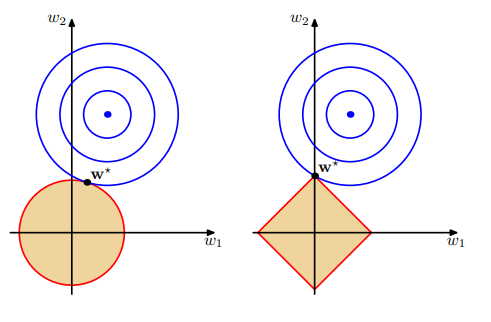
\includegraphics{figures/L1vsL2.PNG}
\caption{Visualization of the impact of the regularization term on the optimization solution. The blue contours plot represents regularized cost function along with a $L2$ (left) and $L1$ (right) regularization terms. The optimum value of the parameters is denoted by $w^{*}$. The lasso regularization gives a spare solution in which $w_{1}^*=0$. Figure taken from \cite{bishop}  
\label{fig:L1vsL2}}
\end{figure}
The statistical justification of using both $L1$ and $L2$ regularization comes from Maximum A posterior Estimation (MAP), which enhance the maximum likelihood method by adding prior factor. The MAP framework is one of the tools of the Bayesian statistic, which allows adding a probability distribution over the model's parameters (external heuristics). From a conceptual standpoint, the interpretation is that one has some prior knowledge about the possible values of the unknown parameters (for instance a physics law such as momentum conservation).

\paragraph{Logistic Regression and data linear separability} \mbox{}
\\

The logistic regression model has zero training error rate only when the data is linearly separable, which means that there is an n-dimensional hyperplane that can separate data into classes. Figure \ref{fig:linear separability} presents example of such a data.



\begin{figure}[!h]
\centering
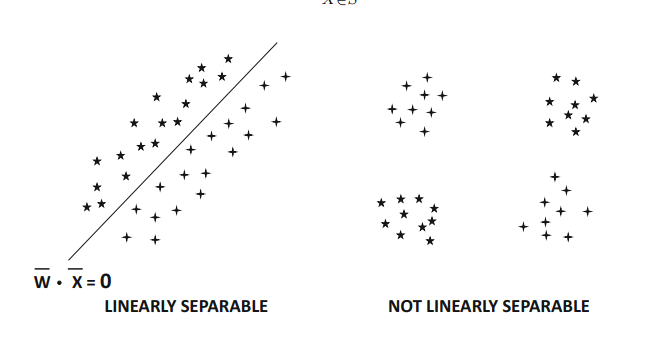
\includegraphics{figures/limear_separability.PNG}
\caption{Visualization of the linear separability of a data.  
\label{fig:linear separability}}
\end{figure}


The linear separability of the data is a strong assumption and, in practical applications, holds rarely. To produce the nonlinear decision boundaries, two methods can be used. The first one is to handcraft a function $\phi(x)$ that transforms data into the form that makes it linearly separable. This task is very challenging, taking into consideration the high dimensionality of the practical classification problems. The second idea, discussed in the next sections, is to build a classifier that can generate nonlinear classification rules. 

\begin{figure}
  \centering
  \begin{tabular}{@{}c@{}}
    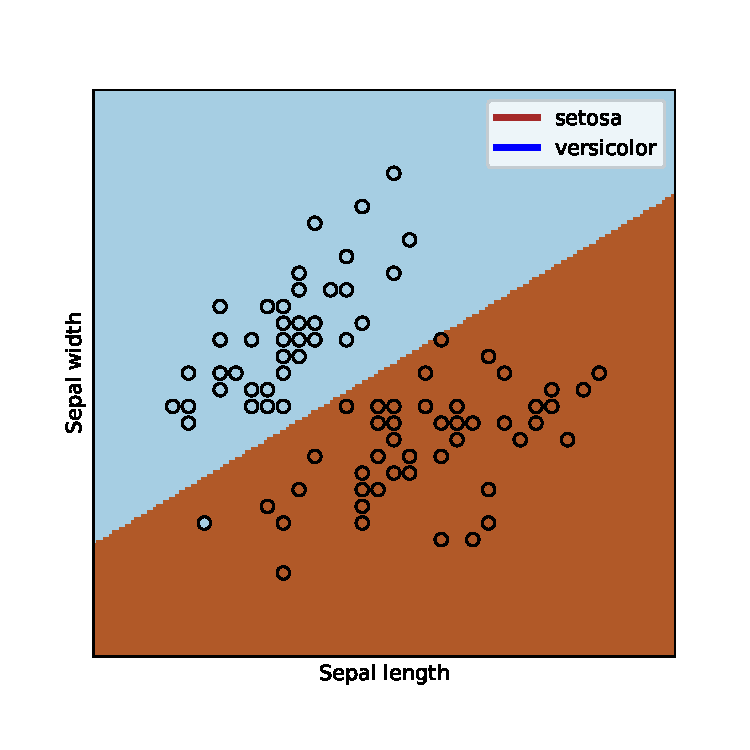
\includegraphics[width=0.6\linewidth]{figures/decision_boundaries_lr.pdf}
  \end{tabular}

  \vspace{\floatsep}

  \begin{tabular}{@{}c@{}}
    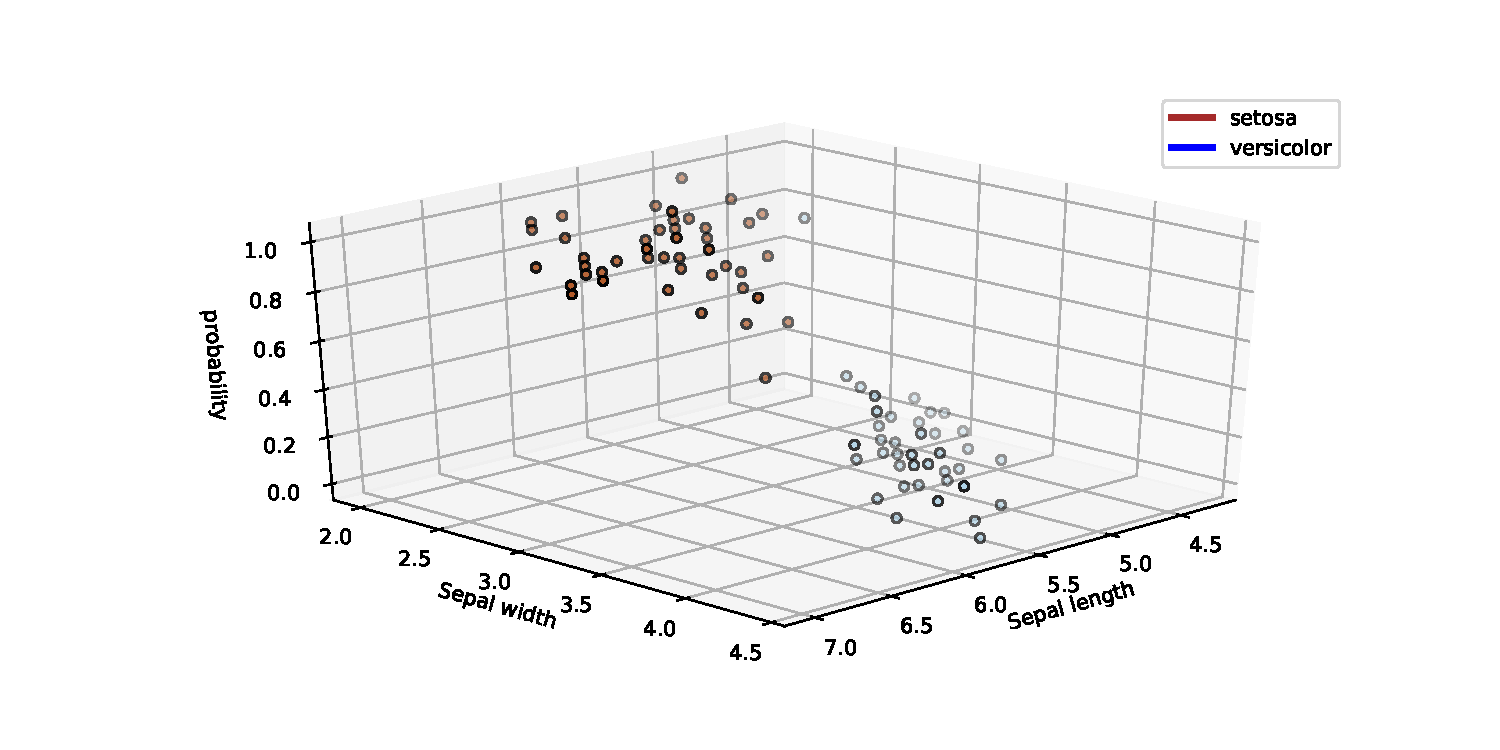
\includegraphics[width=\linewidth]{figures/3D_log_reg.pdf}
  \end{tabular}

  \caption{Logistic regression decision boundaries. The bottom figure presents a 3D plot, which visualize the classifier output (horizontal line) versus feature values.  
\label{fig:LRdecision boundary}}  
\end{figure}



\subsection{XGboost Classifier}
\label{sec:xgboost}
The XGboost stands for Extreme Gradient Boosting \cite{xgboost}. It is the state-of-the-art implementation of the Gradient Boosted Classifier. The Gradient Boosted Classifier is a model that uses $k$ additive functions to predict the output.  
Each of these functions is called a weak learner. The next section discusses one of the usual choice of week learner - Decision Tree Classifier. 


\subsubsection{Decision Tree Classifier}
\label{sec:Decision_Trees}
The Decision Tree Classifier is a parametric model implemented by recursively partitioning the input space, and defining a local model in each resulting region of input space. This can be represented by a so-called tree object, with one leaf per region. 
Analytically, the model can be expressed in the following form: 

\begin{equation}
    f(x) = \sum^{L}_{l=1} \gamma_l \mathds{1}(x \in \mathcal{R}_{l})
\end{equation}

where: $L$ is the number of disjoint regions $R_{1},R{2}, \ldots, R_{L}$ of the entire input space, $\gamma_l$ is a local response for region $R_l$, and $x$ is a input N-dim vector. The decision whether to make an additional split is based on the information gain metric. The information gain is closely related to the information entropy \ref{eq:entropy}: 

\begin{equation}
    IG(P,a) = H(P) - H(P|a)
\end{equation}

% buba - opis poniżej jest trudny do zinterpretowania - czym jest atrybut a?
% warto dodać, że celem algorytmu jest maksymalizacja entropii w każdym obszarze
% co interepretujemy jako istnienie w tym obszarze "identycznych obiektów"

where $ H(P|a)$ is the conditional entropy of $P$ given the value of the attribute is $a$. The information gain can be interpreted as a change in the entropy when attribute $a$ is observed. The process of the partitioning of the input space is performed by the procedure, in which greedy selects the attribute that gives the highest information gain. 
From the practical perspective, Decision Tree (DT) algorithm is implemented in the following way:

\begin{algorithm}[caption={Building Decision Tree (psudocode)}, label={DTAlgorithm}]
Data : Training attribute-value dataset $D$
Tree = {}
if all instance in $D$ has the same class $c$ then:
   label(Tree) $\leftarrow c$ 
   terminate
else if attributes set $= \emptyset$ or no attributes has positive information gain then:
   label(Tree) $\leftarrow $ most common class in $D$
   terminate
for all attributes $a \in D$ do:
   $a_best$ = Best attributes according to the information gain
   Tree = create decision tree node with $a_best$ as a root
   $D_a$ = Induced sub-dataset from $D$ based on $a_best$
   for each value of attributes in $D_a$ :
      $Tree_{a}$ = BuildDecisionTree($D_a$)
      attach  $Tree_{a}$  to the corresponding branch Tree
end for
return Tree
\end{algorithm}

\begin{figure}%
    \centering
    \subfloat{{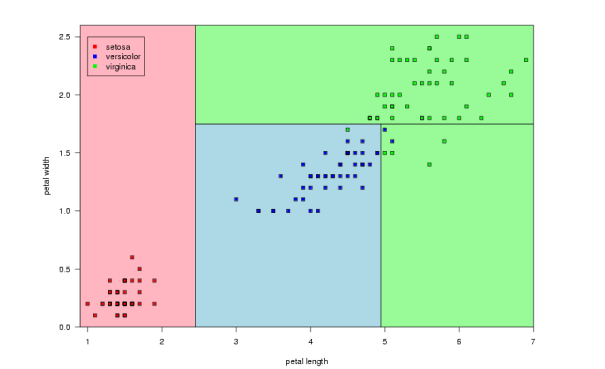
\includegraphics[clip,width=\columnwidth]{figures/DTBoundaries.PNG} }}%
    \qquad
    \subfloat{{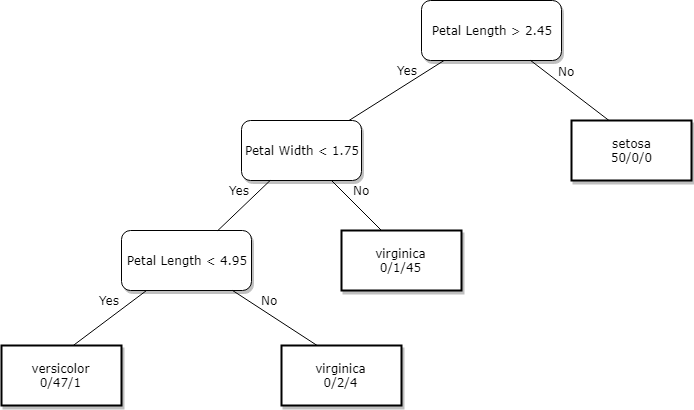
\includegraphics[clip,width=\columnwidth]{figures/DecisionTreeStructure.png} }}%
    \caption{Example of the result of training a DT Classifier based on the Iris dataset \cite{fisher} \cite{anderson}. This dataset consists of three different species of iris plant. The upper figure present the decision boundaries that are produced by the classifier, each of the color represents different species of iris. The graph below, shows the nodes where the decisions are evaluated by the classifier. The decision boundaries plot was taken from \cite{DecisionTrees}. }%
    \label{fig:Decision Tree}%
\end{figure}

Figure \ref{fig:Decision Tree} presents the exemplary DT Classifier, that was trained in order to classify different spices of iris plant \cite{fisher} \cite{anderson}. It is visible that each node of the tree is composed of a single "yes or no" type question, and the prediction is calculated by recursively answering those questions (starting from the root node) using the information decoded within the input vector. One of the most critical features of this model is that a human easily interprets its prediction. One can get the intuition of why the model made a particular decision by looking at each question-answer pair and comparing them with an initial problem's domain knowledge. The DT models are very popular in the field of High Energy Physics.

\subsubsection{Gradient Boosting}

Gradient Boosting is an idea to enhance a single weak learner prediction by creating an ensemble of those models. The gradient boosted method creates a strong learner model by learning from the errors of the weak learners. Typically, the weak learner is selected to be a shallow DT or Logistic Regression model. Although all classification models can be used, the only regiment is that the weak learner needs to perform better than chance when trying to label the data.     

Gradient Boosting constructs additive model by sub-sequentially fitting week learners to current pseudo residual at each iteration\footnote{one \textbf{iteration} is a process of adding one weak learner to the model}. Mathematically, the Gradient Boosting algorithms minimize the cost function by approximating the optimal solution $f^*(x)$ using an additive expansion of the form:
\begin{equation} 
    f(\textbf{x}_i) = \sum_{k=0}^{K} f_k(\textbf{x}_i; w, q, T)
\end{equation}

Where $f_k(\textbf{x}; w, q, T)$ is a weak learner belonging to the class of regression trees, $q$ represents the structure of each tree that maps from input vector $\textbf{x}$ into the corresponding leaf index, $T$ is a number of leaves in each tree and $w \in \mathcal{R}^{T}$ is a leaf weight. To learn the parameters of each function that constitutes the xgboost model, the following cost function is minimized:

\begin{equation}
\label{eq:xgboost_loss}
\begin{split}
    \mathcal{L}_{xgboost}(f) &= \sum_{i=0}^{N} \mathcal{L}(y_i, f(\mathbf{x}_i)) + \sum_{k=0}^{K}\Omega(f_{k})  \\ 
&= \sum_{i=0}^{N} \mathcal{L}(y_i, f(\mathbf{x}_i))  + \gamma T +\frac{1}{2}\lambda ||w||^{2}
\end{split}
\end{equation}

where $\mathcal{L}$ is a is a differentiable convex loss function \footnote{Within the scope of this thesis only Cross-Entropy was tested, although section \ref{sec:focal_loss} provides description of an alternative metric.} that measures the difference between the prediction $f(\vec{x_i})$ and the target $y_i$. 
The term $\Omega$ penalizes the complexity of the model and depends on two hyperparameters. The first one $\gamma$ is dedicated to reducing the number of leaves, and $\lambda$ is $L2$ regularization parameter. 

The optimization of the formula \ref{eq:xgboost_loss} is infeasible because it introduces functions as parameters, and that why using numerical methods such as Stochastic Gradient Descent is not an option since they operate on numerical vectors, not trees. Instead, the model is trained in an additive manner, each time a single decision tree is added to the model. Let $\hat{y}_{i}^{(t)}$ be the model's prediction of the $i$-th training instance at the $t$-th interaction, then this procedure can unfold:        

\begin{equation}
\begin{split}
    \hat{y}_{i}^{(0)} &= 0  \\
    \hat{y}_{i}^{(1)} &= f_{1}(\textbf{x}_i) = \hat{y}_{i}^{(0)} +  f_{1}(\textbf{x}_i)  \\
    \hat{y}_{i}^{(0)} &= f_{1}(\textbf{x}_i) + f_{2}(\textbf{x}_i) = \hat{y}_{i}^{(1)} +  f_{2}(\textbf{x}_i)   \\
    & \vdots   \\ 
    \hat{y}_{i}^{(t)} &=  \sum_{k=1}^{t}f_{k}(\textbf{x}_i) =  \hat{y}_{i}^{(t-1)} + f_{(t-1)}(\textbf{x}_i)
\end{split}
\end{equation}

The cost function \ref{eq:xgboost_loss} can be expressed as:

\begin{equation}
   \mathcal{L}_{xgboost}^{(t)} = \sum_{i=0}^{N}  \mathcal{L}(y_i,  \hat{y}_{i}^{(t-1)} + f_{t}(\mathbf{x}_i)) + \Omega(f_{t})
\end{equation}
 
Using the Taylor expansion formula for the objective, the loss function can be written as:

\begin{equation}
\begin{split}
   \mathcal{L}_{xgboost}^{(t)} &\simeq \sum_{i=0}^{N} \left[ 
   \mathcal{L}(y_i, \hat{y}^{(t-1)}) + g_i f_t(\mathbf{x}_i) + \frac{1}{2}h_if_{t}^{2}(\mathbf{x}_i)  
   \right] + \Omega(f_{t}) \\
    &\simeq \sum_{i=0}^{N} \left[ 
 g_i f_t(\mathbf{x}_i) + \frac{1}{2}h_if_{t}^{2}(\mathbf{x}_i)  
   \right] + \Omega(f_{t})
   \end{split}
   \label{eq:xgboost_taylor}
\end{equation}

where $g_i$ and $h_i$ are gradient and hessian defined as follow:  
\begin{equation}
    g_i = \left[\frac{\partial \mathcal{L}(y_{i},\hat{y}^{(t-1)})}{\partial \hat{y}^{(t-1)}} \right]
\end{equation}

\begin{equation}
    h_i = \left[\frac{\partial^2 \mathcal{L}(y_{i},\hat{y}^{(t-1)})}{\partial \hat{y}^{(t-1)}} \right]
\end{equation}

Learning objective written in the form of \ref{eq:xgboost_taylor} is very convenient from the perspective of the code implementation. To add customized loss function, one needs to provide the implementation of the gradient and hessian. The procedure, that minimize \ref{eq:xgboost_taylor} is visualized in figure \ref{fig:GB_visualization}. 

\begin{figure}
\centering
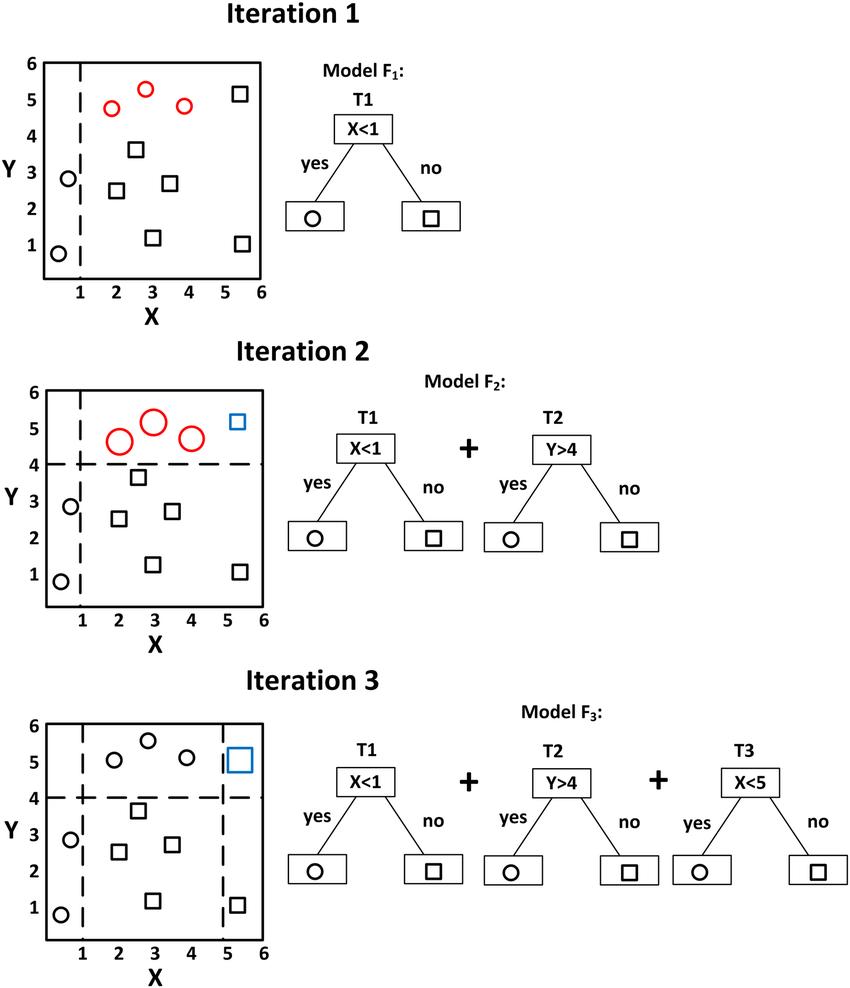
\includegraphics[scale=0.8]{figures/GB_visualization.png}
\caption{Gradient boosting algorithms visualization. Each iteration corresponds to adding one tree, which allows creating more sophisticated non-linear decision boundaries. 
This graph was taken from \cite{GB_visualization}
\label{fig:GB_visualization}}
\end{figure}
  
XGBoost is a perfect combination of software and hardware optimization techniques to yield superior results using less computing resources in the shortest amount of time. The main features of this package are listed below: 
% nazwa xgboost jest używana niekonsystentnie
\begin{itemize}
    \item \textbf{Split finding approximate algorithm} To find the best split over a continuous feature space, data need to be sorted and fit entirely into memory. This may be a problem in the case of large datasets.
    An approximate algorithm is used for this. Candidate split points are proposed based on the percentiles of the feature distributions.
    \item  \textbf{Sparsity-aware algorithm}. The input may be sparse due to such reasons as one-hot encoding, missing values, or zero entries. XGBoost is aware of the sparsity pattern in the data and visits only the default direction (non-missing entries) in each node.
    % hmm, trzeba to wyjaśnić...
    \item  \textbf{Out-of-core computation} 
    Data that do not fit into main memory is divided into multiple blocks, and each block is stored on the disk. A dedicated algorithm can compress each block by columns and then decompress it on the fly.
    \item \textbf{Regularized Learning Objective} The default loss function is composed of two components 
    \begin{equation}
        \mathcal{L}_{xgboost}(w) = \mathcal{L}(w) + \Omega(w)
    \end{equation}
    where $\Omega(w)$ is a  regularization term and depends on the complexity of the model. Most of the implementations, including TMVA \cite{TMVA}, miss this term and thus they are more prone to overtraining. 
\end{itemize}


\subsection{Deep Neural Network}
\label{sec:DNN}
This section provides a basic intuition on how the Deep Neural Network works. The one who wants to know more should refer to \cite{DLBook}.  

The critical limitation of linear models described in section \ref{sec:LogReg} is a lack of ability to generate non-linear decision boundaries. To overcome this limitation, a mapping $\varphi(\vec{x})$ that transforms the input vectors into the representation that makes those vectors linearly separable has to be found. The most robust strategy of searching for such transformations is to construct a model that will be capable of learning $\varphi(\vec{x})$. One of such a model is a neural network, which parametrizes $\varphi(\vec{x};\theta)$ and uses the gradient-based optimization algorithm to find the optimal set of $\theta$ that corresponds to the desired representation. The idea of such a model comes from the brain's computation mechanism \cite{NN_brain}, which consists of computation units called neurons. The schematic view of such a model is presented in figure \ref{fig:NN}. 

 A neuron is an entity that multiplies each input by its weight and sums them, afterwards applies a non-linear function to the result. The non-linear function is a crucial feature of the whole neural network idea, which is indicated in figure \ref{fig:NN} by the sigmoid shaped symbol. Its absence would not allow creating a more complex model that the logistic regression.  The neurons are connected, forming a network, in which the output of a neuron is feed into the inputs following neurons. Neural network models arrange the neurons into layers, which reflect the flow of information. Within the scope of this thesis, only models built on top of fully-connected layers were investigated. Such a layer applies an affine transformation to the input vector \footnote{Typically, that kind of layer is called linear, which can be misleading since it applies an affine transformation, not a linear one}. Therefore, the output of the first layer can be written as: 

\begin{equation}
h^{(1)} = \sigma^{(1)}(w^{(1)T}\vec{x}+b^{(1)})
\end{equation}
and the output of the  second layer is given by: 
\begin{equation}
h^{(2)} = \sigma^{(2)}(w^{(2)T}h^{(1)}+b^{(2)})
\end{equation}
where $  \sigma^{(i)}$ is an $i$-th activation function, $\vec{x} \in \mathcal{R}^{in}$, $w^{(i)} \in \mathcal{R}^{d_{i-1}\times d_{i}}$ are weights matrix, $b^{(i)} \in \mathcal{R}^{d_{i}}$ is a bias term and $d_{i}$ is the number of neurons in the $i$-th layer.  

Propagation of the input vector $\vec{x}$ through the network by iteratively calculating the output of each hidden layer to produce the prediction $\hat{y}$ is called \textbf{forward propagation}, see algorithm \ref{alg:forward_prop} for implementation details. Beside of providing the prediction, the full version of the forward propagation contains loss calculation step.  

As indicated in figure \ref{fig:NN}, the bottom layer, which has no incoming arrows, is the input to the model, where each neuron represents one component of the input vector $\vec{x}$. 
 The top-most layer has no outgoing arrows. Thus, it is the output of the network.  The layers situated between the input and the output are called \textbf{hidden}. 

\begin{algorithm}[caption={Forward propagation of feed-forward neural network }, label={alg:forward_prop}]
Require: Training data ${x^{train}_{i} , y_{i}}$;
Require: Network of depth $l$;
Require: $W^{(i)} \textrm{and}  b^{(i)}, i \in \{ 1, \ldots l \}$ the weight matrices and bias vectors of the model
$h^{0} =x^{train}_{i}$ 
for $k = 1, \ldots, l$ do
   $z^{(k)} = W^{(k)}h^{k-1} +b^{(k)}$ 
   $h^{(k)} = \sigma^{(k)}(z^{(k)})$
end for
$\hat{y} = h^{l}$
$\mathcal{L} = L(y_{i}, \hat{y}) + \lambda \omega(w, b)$
\end{algorithm}

\begin{figure}[!ht]
\centering
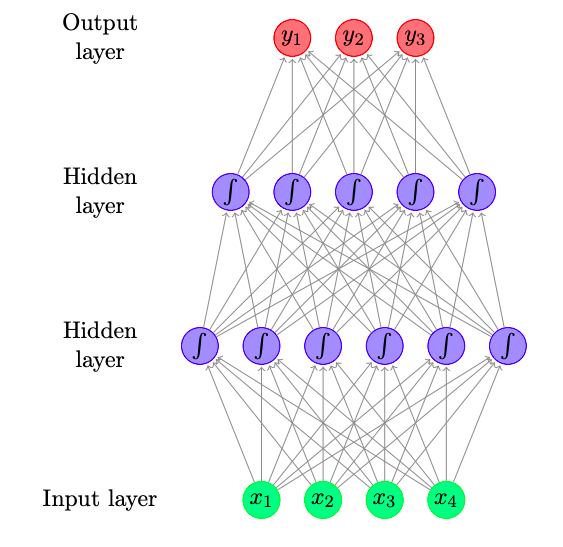
\includegraphics[scale=0.7]{figures/NN.png}
\caption{ Feed-forward neural network with two hidden layers.  Each circle represents a neuron, with incoming arrows being the neuron’s inputs and outgoing arrows being the neuron’s outputs. Each arrow carries a weight, reflecting its importance (not shown). Figure taken from \cite{text_processing}.
}
\label{fig:NN}
\end{figure} 
 
 
The non-linear function $\sigma$ can be implemented in a various ways. The design of it is an extremely active research area. The two most popular types of activation functions are sigmoid, described in section \ref{sec:LogReg}, and rectified linear unit (ReLU) (both were used to train the model within the presented studies).

ReLU \cite{relu} it defined as follow: 

\begin{equation}
ReLU(x) = max(0,x)= \left\{ \begin{array}{ll}
x & x>0\\
0 & \textrm{otherwise}\\
\end{array} \right.
\end{equation}

This activation function is the default activation function recommended for use inside hidden layer for most feed-forward neural networks \cite{DLBook}. Applying this function to the output of a linear transformation yields a non-linear transformation, which remains very close to linear. The only difference between a linear unit and a rectified linear unit is that a ReLU unit outputs zero across half its domain. 

One of the essential features of this activation function is the fact that its derivative is not computationally expensive and remains large whenever the unit is active. On the other hand, the drawback of the ReLU units is that they cannot learn via gradient-based methods on examples for which their activation is zero.
This issue was addressed by Leaky ReLU \cite{LeakyReLU} and PReLU \cite{PReLU}. 

\subsection{Universal Approximation Theorem}

One of the most important concepts of the neural networks with at least one hidden layer is the capability of approximating any Borel measurable function \footnote{Within the scope of this thesis, a function is Borel measurable when it is continuous on a closed and bounded subset of $\mathcal{R}^{n}$}. This observation is called the universal approximation theorem. The proof of this theorem is beyond the scope of this thesis and can be found in  \cite{Universal_approx_1} and \cite{Universal_approx_2}. The intuition behind this theorem is shown in figure \ref{fig:Universal_approx}.
The theorem does not say how to construct the network; therefore the layer may be infeasibly large and may fail to learn and generalize correctly. From a practical perspective, it is recommended to use deeper (having more layers) rather than wider networks \cite{Relu_regions}. 

\begin{figure}[!htb]
 \begin{center}
   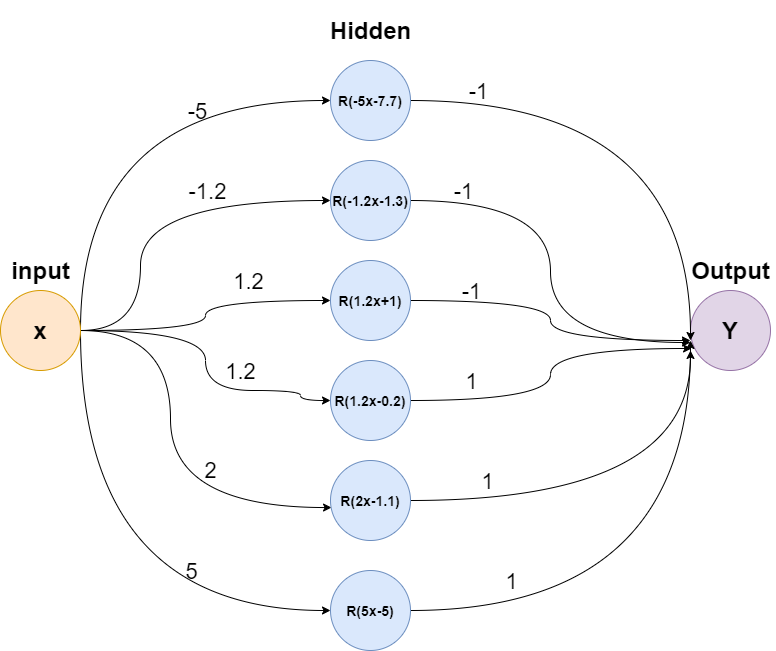
\includegraphics[width=0.7\linewidth]{figures/UAT_2.png}\\
    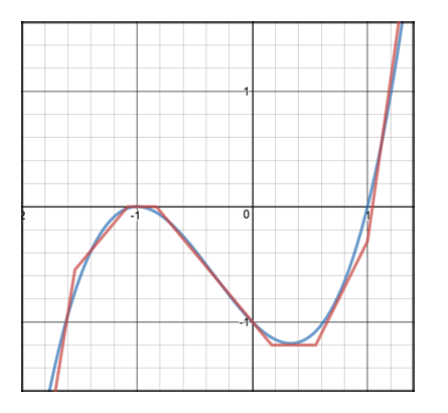
\includegraphics[width=0.7\linewidth]{figures/UAT.PNG}
   \caption[Visualization of the Universal Approximation Theorem]{Visualization of the Universal Approximation Theorem. The objective was to build a network with one hidden layer that is able to represent $f(x)= x^{3}+x^{2}-x-1$. This network is presented in the left plot. The right plot present the $f(x)$ and weighted sum of six ReLU functions. To reduce the approximation error more ReLU functions has to be added. Figure adapted from \cite{UAT_blog}
     \label{fig:Universal_approx}}
 \end{center}
\end{figure}

\subsubsection{Back-propagation and computational graphs}
The remainder of this section is dedicated to present the algorithm that is widely used to train the neural network model. It contains three steps: 

\begin{itemize}
    \item Forward propagation with loss calculation;
    \item Calculation of the loss function with respect to the model's weights;
    \item Weight update via Gradient Descent-like algorithm using the previously calculated gradient.
\end{itemize}

This procedure was designed to iteratively adjust the weights of connected neurons using the cross-entropy between the network's output vector and the desired one. As a result of this procedure, the hidden units produce a new feature's representations, which are more convenient from the downstream task perspective.  To estimate the change of weights for each layer, their gradient has to be calculated first. This algorithm is called \textbf{backpropagation} or backprop and was proposed in 1986 by G. Hinton \cite{backprop}. 
The final round of evaluating a single step in training deep neural networks is to use the previously calculated gradients to update the model's weights using Gradient Descent-like algorithm. 

\begin{algorithm}[caption={Backward propagation of feed-forward neural network }, label={alg:backward_prop}]
Require: Training data ${x^{train}_{i} , y_{i}}$;
Require: Network of depth $l$;
Require: $W^{(i)}$ and  $b^{(i)}, i \in \{ 1, \ldots l \}$ the weight matrices and bias vectors of the model

run forward propagation for a given example $x^{train}_{i}$
compute the gradient on the output layer: 
$g \leftarrow \nabla_{\hat{y}} \mathcal{L} =  \nabla_{\hat{y}} \mathcal{L}(y, \hat{y})$ 
for $k = l-1, \ldots, 1$ do
   convert the gradient on the $k$-th layer output into a gradient on the pre-$\sigma$ activation: 
   $g \leftarrow_{z^{(k)}} \mathcal{L} = g \odot \sigma'(z^{(k)})$
   compute gradients on a weight and biases:
   $\nabla_{b^{k}} \mathcal{L}  = g + \lambda \nabla_{b^{k}} \Omega(W, b) $ 
   $\nabla_{W^{k}} \mathcal{L}  = g z^{(k-1)T} + \lambda \nabla_{W^{k}} \Omega(W, b) $ 
   propagate the gradients w.r.t the next lower-level hidden layer activation:
   $g \leftarrow_{z^{(k-1)}} \mathcal{L} = W^{(k)T}g$
end for
\end{algorithm}

where $\odot$ is a Hadamard Product also known as element-wise product defined as:

\begin{equation}
    (A \odot B)_{ij} = (A \odot B)_{ij} = (A)_{ij} (B)_{ij}
\end{equation}

The backprop, which is demonstrated by the algorithm \ref{alg:backward_prop} is specified to the feed-forward neural network only. However, the modern deep learning framework, such as TensorFlow \cite{tensorflow} or PyTorch \cite{pytorch}, is based on a general form of backpropagation, which is implemented using computational graphs. 
A computational graph is a graph in which each node represents a variable. The variable may be a scalar, matrix,  tensor \footnote{In the field of deep learning, a tensor is an object that has more than two dimensions and, in contrary to the tensor in physics, does not need to follow any transformation rules.} or variable of another type which is useful when calculating higher-order derivations.    
The edges of the graph represent the operations that are applied to particular nodes. The direction of the edge indicates whether some node is a parent of a given child node. 
One of the approaches to calculating the gradient is to extend the graph by adding additional nodes to the graph that provide a symbolic description of the desired derivatives. A detailed explanation of how the PyTorch implements gradient calculation can be found in \cite{autograd}. 

From the practical perspective, the one who wants to build a model using the PyTorch framework has to define only how the forward propagation is calculated. The framework will take care of backward propagation.

\begin{figure}[!ht]
\centering
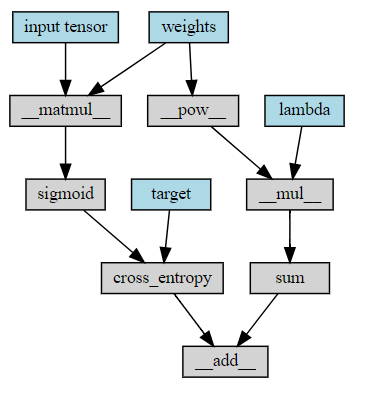
\includegraphics[width=0.7\textwidth]{figures/Comput_graph_2.PNG}
\caption{Computational graph used to perform the forward propagation and estimate the cross-entropy loss with L2 regularization for a single layer full-connected neural network. The blue rectangles represent tensors and the gray operations applied on those tensors. Figure generated by author's implementation of the autograd tool.
}
\label{fig:Comput_graph}
\end{figure} 

\subsection{Hyperparameter optimization}
\label{sec:hyperparameters}

The model's hyperparameter is a non-learnable parameter that has to be set priory to the whole training process. Each of the models has its own set of hyperparameters, which depends on the model's architecture. For instance, one of the hyperparameters of the Decision Tree, described in section \ref{sec:Decision_Trees} is its maximum depth, which indicates what the maximum number of splits used to construct the tree is. 

One of the essential concepts regarding the hyperparameters is that its influence on the model's performance is not equal. Some of the hyperparameters are more important than the others. Additionally, the interaction between each of the hyperparameters is usually unknown and complex. 

Hyperparameter optimization is a procedure of searching for a set of hyperparameters to achieve high prediction accuracy. The wrong choice of the hyperparameters may lead to a significant decrement of the classification power of the model. There are several hyperparameter tuning techniques, but three are presented within the scope of this thesis. The difference among each of the method is a strategy to choose the set of $S$ trial points $\{\lambda^{(1)}, \ldots , \lambda^{(S)} \}$ to evaluate $f(x;\lambda)$ in order to find the $\lambda^{(i)}$ parameters that work the best. Within the scope of this thesis, three methods are explained; see section \ref{sec:GS and RS} and \ref{sec:BayesOpt}.  

\subsubsection{Cross Validation}
One of the methods to get more reliable measurement of the classifier performance is k-Fold cross-validation \cite{Statistical_Methods}, which is schematically shown in figure \ref{fig:CV}. 
This method randomly split the data into k independent subsets. For instance, if $k = 5$, 80\% of data is used to train the model while 20\% of the data sample constitutes the validation set.   

Subsequently, one of the subsets is used to check the model's performance and the reaming data to train it. Each fold generates one prediction. That created set of scores can be used to estimate the statistical uncertainty of the classifier's performance. The cross-validation result is more robust and reliable than a single score calculated on a single test set.   

\begin{figure}[h]
\centering
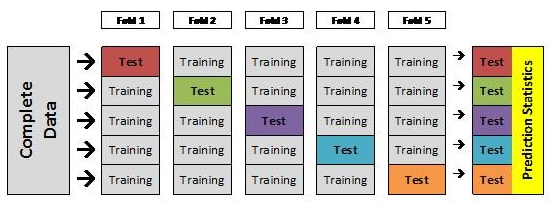
\includegraphics{figures/CV.PNG}
\caption{ The visualization of k-Fold cross validation idea. Figure taken from the internet.
\label{fig:CV}}
\end{figure}

This technique is advantageous when deciding which set of hyperparameters works best. The cross-validation provides a metric performance distribution rather than a single measurement. The drawback of this method is that for more complicated models, which training takes a lot of time, it becomes infeasible.

\subsubsection{Grid and Random Search}
\label{sec:GS and RS}
Grid Search, except for manual search, is the most basic methodology to tune hyperparameters. It splits the hyperparameter space into rectangular hype-regions. Each of the regions represents one trial. In other words, Grid Search choose a set of values per each variable $(\lambda_{1} \ldots \lambda_{K})$, where $K$ is a number of hyperparameters, and then a set of trials is formed by assembling every combination of values for each hyperparameter; therefore the number o trials in a Grid Search is:
\begin{equation}
    S=\prod^{K}_{k=1}|\lambda_{k}|  
\end{equation}

This product over $K$ hyperparameters makes Grid Search suffer from the curse of dimensionality because the number of joint hyperparameters values, that has to be checked grows exponentially with the number of hyperparameters. 

\begin{figure}
\centering
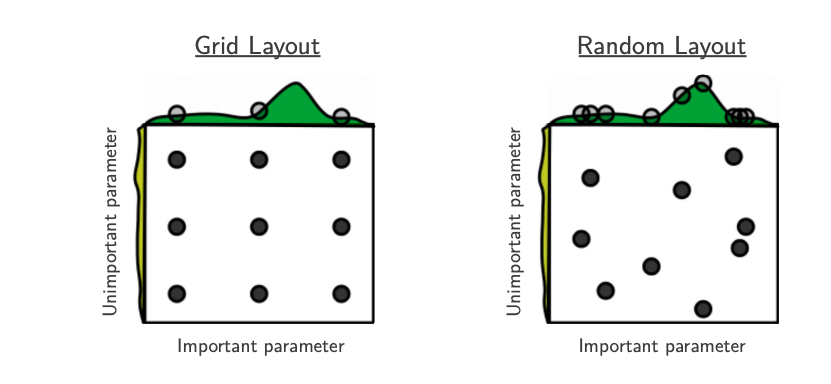
\includegraphics{figures/GridSearch.png}
\caption{Comparison of the Grid Search and Random Search methods of hyper-parameters tuning. 
On both of the figures, the x-axis represents a hyper-parameter. The modification of its value has a negligible effect on model performance, and the y-axis presents a hyper-parameter that has a large impact on the model classification ability \cite{RandomSearch}. 
\label{fig:GridSearch}}
\end{figure} 

The only real difference between Grid Search and Random Search is on step 1 of the strategy cycle – Random Search picks the point randomly from the configuration space. 
The researcher needs to provide a set of distributions, one per hyperparameter, to generate trials. From a practical perspective, the usual choice for these distributions is uniform and log-uniform distributions. The second one is a common choice when dealing with such hyperparameter as the learning rate, where the hyperparameter's value range that needs to be check is   $ \lambda_k \in (1\times 10^{-6},1)$. 


To compare these two methods a toy experiment was shown in figure \ref{fig:GridSearch}. It presented a search for nine trials for optimizing a function \\ $f(x,y) = g(x) + h(y) \approx g(x)$. With Grid Search, nine trials test $g(x)$ in three distinct places only, in comparison Random Search leveraged all nine trials to explore distinct value of $g(x)$. The failure of Grid Search is the rule rather than the exception in high dimensional hyperparameter optimization \cite{RandomSearch}. 

\subsubsection{Bayesian optimization}
\label{sec:BayesOpt}
Both of the previously described methods have one drawback. Neither of them leverages the previous evaluation results to reject the regions where there is a small probability of finding the maximum value of the unknown objective function $f(x)$, which is a nonlinear function defined over a compact set $\mathcal{A}$. This section is dedicated to describing the general idea of Bayesian Optimization, which can be applied to any regression problems. It is not limited to the optimal hyperparameter search. The enhancement to these methods should make use of accumulated observations $D_{1:t} = \{ x_{1:t}, f(x_{1:t}) \}$, where $x_i$ is a $i$th sample, and $f(x_i)$ is a observation of the objective function at $x_i$.   \footnote{In the case of hyperparameters optimization, $f$ is a specific metric used to measure model performance, within this thesis, the ROC AUC was selected,  and $x$ represents a vector of hyperparameters }. One of the methods that fulfil this condition is Bayesian optimization.  
 
Bayesian optimization is a technique widely used for solving the regression problems when function evaluation is expensive, and the derivative is usually unknown. Thus the usual optimization methods like Gradient Descent, are not applicable. The hyperparameter optimization problem belongs to this area. To be more precise, in the case of seed classification model training takes a significant amount of time (in the case of XGboost, one trial takes more than an hour), and the model performance derivative with respect to, for instance, the tree depth is not defined.    
% buba - czy to jest dla naszego trackingu? To trzeba dopisać
% AD: fixed (I hope so). 
The method's name comes from the famous Bayes theorem. In the case of an optimization problem, the posterior distribution can be expressed in the following manner: 

\begin{equation}
\label{eq:BO_posteriori}
    P(f|D_{1:t}) \propto P(D_{1:t} | f) \cdot  P(f)
\end{equation}

where $ P(D_{1:t} | f)$ is a likelihood function, $D_{1:t}$ is a dataset of previous observation that contains $t$  consecutive trials, $P(f)$ is a priory function that express one's belief on a objective function $f$, and  $P(f|D_{1:t})$ is a posterior distribution. The assumption of the Bayesian optimization method is the function $f$ has to be \textbf{Lipschitz-continuous}, which means that exist some constant $C$, such for all pairs $x_1, x_2  \in \mathcal{A}$ the following inequality holds:

\begin{equation}
||f(x_1)-f(x_2)|| \leq C ||x_1-x_2|| 
\end{equation}
% buba - nie wyjaśnione są podwójne nawiasy
% AD: Dodalem oznacznie normy. Zastanawiam się, czy dalej opisywać co to jest norma, jakie warunki spełania etc?   
where  $||\cdot ||$ denotes a norm.


The posterior probabilities capture updated beliefs about the unknown objective function. 
This may be interpreted as a single step of the Bayesian optimization procedure, which is an estimation of the objective function with a surrogate model. The surrogate modelling is a technique which builds the approximating model of the objective function using models that are cheap and fast to evaluate. 

To sample efficiently trails $x$ \footnote{In the case of hyperparameters optimization $x$ corresponds to the vector of hyperparameters $x= (\lambda_1, \lambda_2, \cdots)^{T}$}, Bayesian optimization has the second component - acquisition function $u(x|D_{1:t})$. This function is used to determine the next trial location $x_{t+1}$. The acquisition function should be able to find a trade-off between exploration (searching for a region where the surrogate function is very uncertain) and exploitation (searching for values of $x$ where $f(x)$ is expected to be high), which is shown in figure \ref{fig:BO}. 

\begin{algorithm}[caption={Bayesian Optimization}] 
\label={alg:Bayesian Optimization}
for t = 1,2, .., do:
   Find the next sampling point $x_{t+1}$ by optimizing the acquisition function: $x_t = argmax_x u(x| D_{1:t}) $
   Sample a possibly noisy objective function $y_{t+1} = f(x_{t+1}) + \epsilon_{t+1}$ 
   Augment the data $D_{1:t+1}= \{ D_{1:t}, (x_{t+1},y_{t+1} ) \} $ and update the surrogate function
end for
\end{algorithm}

\paragraph{Gaussian Process} \mbox{}

A popular surrogate model for Bayesian optimization is a Gaussian process. 
A Gaussian Process is a random process where every point $x \in \mathcal{R}^{d}$, where $d$ is a dimensionality of the optimization problem, for the problem of hyperparameter optimization $d$ is equal to the number of hyperparameters taken into consideration during the study, 
is assigned to a random variable f(x). The Gaussian Process can be interpreted as an extension of the multivariate Gaussian distribution to an infinite dimension or distribution over functions. For such a process, any finite combination of dimensions will be a Gaussian distribution. Gaussian Process is completely specified by its mean function $m$ and $k$ covariance function: 

\begin{equation}
    f(x) \sim  \mathcal{N} \left( m(x), k(x,x')  \right)
\end{equation}

Intuitively, the Gaussian Process can be interpreted as a probability function that, for each value of $x$ returns a mean and variance over all possible values of $f$ at $x$, which is shown in figure \ref{fig:GP}.  
\begin{figure}
\centering
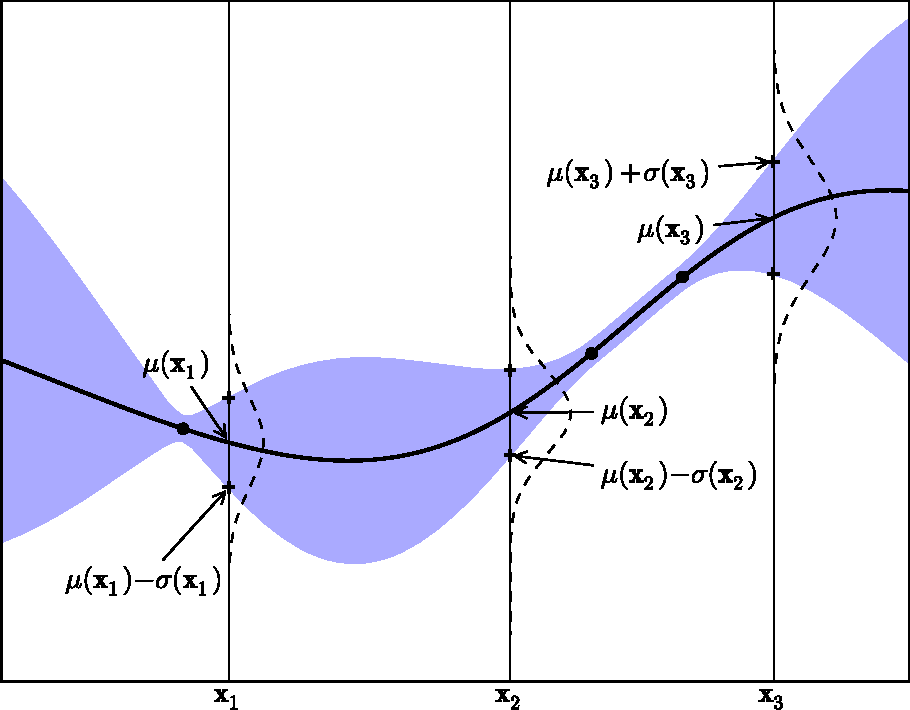
\includegraphics[scale=0.7]{figures/GaussianProcess.png}
\caption{ Simple 1D Gaussian process with three observations $x_{1:3}$. The solid black line is the mean prediction of the Gaussian Process, and the shaded area is one sigma region around mean value.   
Graph taken from \cite{BayesianOpt}.
\label{fig:GP}}
\end{figure}

The convenient and common choice of mean function is $m(x) = 0$ \footnote{ Within the scope of this thesis the Gaussian process is limited to model a noise function in a form of $f(x) = g(x) + \epsilon$ and $\epsilon \sim \mathcal{N}(0, \sigma)$ }. 
The second building block of the Gaussian Process is the covariance function, also called kernel function. The literature discussed several choices of the kernel function, but within the scope of this thesis, only the most popular and basic one is discussed, i.e. squared exponential function: 

\begin{equation}
\label{eq:kernel_function}
    k(x_i,x_j) = exp\left( - \frac{1}{2} ||x_i - x_j||^2 \right)
\end{equation}

The function \ref{eq:kernel_function} approaches $0$ when $x_i$ and $x_j$ get apart and 1 when they are very close to each other. The interpretation of the function is straightforward. When two points are close, they have a significant influence on each other. In the optimization task, the data come from an external model's evaluation and fits the Gaussian Process to get the posterior. In the hyperparameters optimization case, the data refer to the model performance that was training using a particular set of hyperparameters.     
Assuming that the data from the previous iterations is denoted as $\{ (x_{1:t}, f_{1:t}) \}$, the $f(t+1)$ is:

\begin{equation}
\label{eq:GP_priory}
    \begin{bmatrix}
         f_{1:t} \\
         f_{t+1}
        \end{bmatrix}  \sim  \mathcal{N}  \left( 0,  \begin{bmatrix}
         \mathbf{K} & \mathbf{k}  \\
         \mathbf{k}^{T} &  k(x_{t+1},x_{t+1})
        \end{bmatrix}  \right)  
\end{equation}

where 
\begin{equation}
    \mathbf{K} = \begin{bmatrix}
         k(x_{1},x_1) & \ldots  &  k(x_{1},x_t)  \\
          \vdots & \ddots & \vdots \\
           k(x_{1},x_t) & \ldots  &  k(x_{t},x_t)
        \end{bmatrix}
\end{equation}
and
\begin{equation}
    \mathbf{k} = \begin{bmatrix}
        k(x_{t+1},x_1) &  k(x_{t+1},x_2) &  \ldots & k(x_{t+1},x_t) 
        \end{bmatrix}
\end{equation}

Formula \ref{eq:GP_priory} comes from the properties of the Gaussian Process, which states that the joint distribution of Gaussian distributed variables is also a Gaussian. Putting together equations \ref{eq:GP_priory} and \ref{eq:BO_posteriori} one can obtain the expression for the predictive distribution \cite{GaussianProcesses}: 

\begin{equation}
    P(f_{t+1}|D_{1:t, x_{t+1}}) \propto \mathcal{N} (\mu_{t}(x_{t+1}), \sigma_{t}^{2}(x_{t+1}) 
\end{equation}

where: 
\begin{equation*}
\begin{aligned}
    \mu_{t}(x_{t+1}) &= \mathbf{k}^{T}\mathbf{K}^{-1}f_{1:t} \\
     \sigma_{t}^{2}(x_{t+1}) &= k(x_{t+1},x_t) - \mathbf{k}^{T}\mathbf{K}^{-1}\mathbf{k}
     \end{aligned}
\end{equation*}

To summarize Gaussian process allows leverage information obtained from the previous objective function evaluation.


\begin{figure}[!ht]
\centering
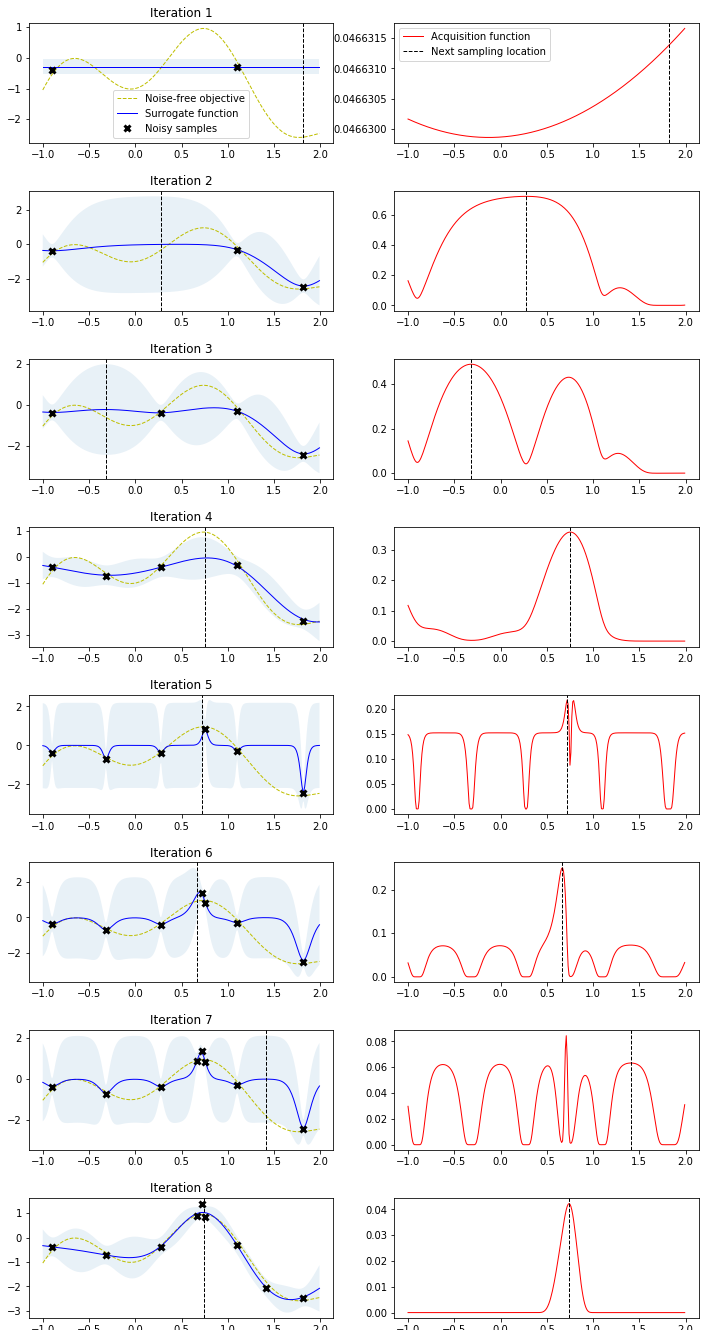
\includegraphics[scale=0.6]{figures/BO.png}
\caption{An example of using Bayesian optimization on a 1D optimization problem - finding maximum of function $f(x)$. 
The figures on the left side show a Gaussian process approximation of the unknown objective function (golden dashed curve) over ten iterations of the sampled value of the objective function. The figures on the right present the acquisition function (red curve). The acquisition function has a high value in the region where GP predicts a high objective, and the prediction uncertainty is high. 
\label{fig:BO}}
\end{figure}

\paragraph{ Acquisition Function for Bayesian Optimization} \mbox{}

This paragraph is dedicated to the second component of Bayesian Optimization, the acquisition function. The role of this object is to drive the search for the optimum solution, see the right side of figure \ref{fig:BO}. It is defined in such a way that its high values correspond to the potentially high values of the objective function. The maximum acquisition function is used to select the next point at which the objective function is evaluated see right side of figure \ref{fig:BO}. A typical choice of the acquisition function is Expected Improvement defined as: 

\begin{equation}
    EI(x) = \mathbf{E}\left(max( f(x)-f(\widetilde{x}) , 0) \right) 
\end{equation}

where $\widetilde{x}$ is best location so far $\widetilde{x} = \underset{{x_i \in x_{1:t}}}{\mathrm{argmax}} f(x_i)$. 

The expected improvement can be evaluated analytically using the Gaussian Process model \cite{GaussianProcesses}: 

\begin{equation}
    EI(x) =   \left\{ \begin{array}{ll}
(\mu(x)-f(\widetilde{x}))\Phi(Z) + \sigma(x)\phi(Z) & \textrm{if $\sigma(x)>0$}\\
0 & \textrm{if  $\sigma=0$}\\
\end{array} \right.
\end{equation}
where $Z= \frac{\mu_{x}-f(\widetilde{x})}{\sigma(x)}-\xi$, $\mu(x)$ and $\sigma(x)$ are the mean and standard deviation of the Gaussian Process posterior predicted at $x$, $\Phi$ and $\phi$ are cumulative distribution function (CDF) and probability density function (PDF) of standard distribution respectively, $\xi$ is the exploration-exploitation trade-off parameter, it is proportional to the amount, understood as a CPU-time or number of iterations, of exploration during optmization. 

% buba co to jest "amount of exploration"? Dla przykładu: w jakich jednostkach
% mierzymy tę zmienną?
% AD: Poprawiłem trochę dodając niewielkie wyjaśnienie. innymi słowami ilość eksploracji rozumiem jako relatywna ilość czasu bądz iteracji, które spędzamy na eksplorowaniu vs ten spedzony na przeszukiwaniu regoinu, w którym spodziewamy sie, że jest maksimum. 
% Przykładowo w Reinforcement Learningu bardzo znacząca jest stratego nazywana \epslion greedy. Wh której z prawdopodobienstwem \epsilon wybieramy losowa akcje oraz z (1-\epsion) wybieramy tę, którą daje nam najlepszą (oczekiwaną) przyszłą nagrodę (reward). Czyli przykładowo jak gramy w Mario (NES) i stoimy na rurze w takim miejscu naciśniemy z prawdopodobienstwem (1- \epslion) przycisk w prawo gdyż spodziewamy się że dzięki temu posuniemy się bliżej w kierunku zamku. Natomiast losowa akcja "w dół" pozwoli nam odkryć skrót. Losowa akcja "lewo, góra" dają nam negatywną nagrodę, gdyż tracimy czas. 
\subsection{Model interpretation}

One of the crucial problems when building \footnote{in this context model building is understood as a complete model selection and validation processes} a complex Machine Learning model is lack of interpretability of its prediction. This fact raises the question of why one should trust the prediction that model gives. The Machine Learning model's interpretability is an active research area, and many ideas were recently published. To make sure that the model, that was trained to classify the track seeds provide reliable predictions two methods, apart from the usual quality metrics,
%except measuring overall statistics\footnote{in this context overall statistic is understood as a single number that was calculated based on a whole validation or test set.}, 
% AD: Czy napewno chcemy to usunąć? Wydaje mi się dość intereujące zadresować różnice poniędzy 
% metrykami globalnymi oraz "lokalnymi" dla pojedynczego przypadku. 
were proposed: LIME (Local Interpretable Model-Agnostic Explanations) \cite{lime} and SHAP (Shapley Additive exPlanations) \cite{shap}. This section starts by presenting a brief overview of both methods. Section \ref{sec:interpretability} resents the results obtained in order to understand the prediction of the trained seed classifier.
\subsubsection{LIME - Local Interpretable Model-Agnostic Explanations }
\label{sec:lime}
The discussion of the LIME should start from choosing models, that are human interpretable. An interpretable explanation needs to use a representation that is understandable to humans, regardless of the actual model's architectures or features used to make a decision. For instance, a possible interpretable representation of the text classification is a vector of binary values indicating the presence or absence of a certain word, even though the model may use more complex input features.
%such as word embedding
%\footnote{word embedding is a collective term for models that learned to map a set of words to a vector of numerical values. The expected properties of such mapping are the words that have a similar meaning are represented by vectors lying close to each other. Moreover, it allowing to use vector arithmetic to work with analogies for instance: $\overrightarrow{king} - \overrightarrow{man} + \overrightarrow{woman}= \overrightarrow{queen}$}. 
%AD: Czy chcemy to wyrzucać? celem tego paragrafu jest zaadresowanie, że wejściem do modelu nie koniecznie musi byc "surowy" wektor cech a moze byc cos bardziej skomplikowanego jak wynik WordEmbeddings (po polsku zanurzenie - kto to tłumczenie wymyślił?! ). Przy okazji tłumaczę tutaj jego idee. 
To get a better intuition of what is the purpose of the LIME explanation, let consider a toy example where a Machine Learning model has to predict whether the patient has the flu or not. The input to this model is the patient's symptoms and other features such as weight or age. LIME selects the symptoms in the patient's history that are most relevant and led to the prediction. With these approximations and the domain knowledge, the doctor can make an informed decision about whether to trust the model's prediction or not. The visualization of this toy experiment is presented in figure \ref{fig:LIME_doctor}.

\begin{figure}[!htb]
\centering
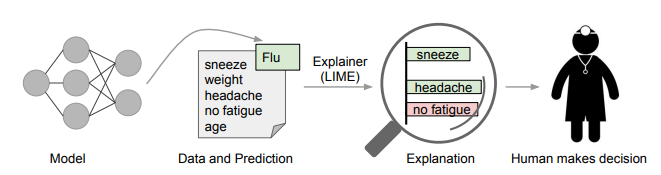
\includegraphics{figures/lime_doctor.PNG}
\caption{A toy example that visualizes the concept of LIME individual prediction explanation. A model predicts that a patient has the flu, and LIME highlights the symptoms in the patient's history that led to the prediction. Sneeze and headache are portrayed as contributing to the "flu" prediction, while "no fatigue" is evidence against it. Figure taken from \cite{lime}.
\label{fig:LIME_doctor}}
\end{figure} 

In the case of the tabular data, the model that can be used as an interpretable approximation is a linear model \footnote{the second type of interpretable model class is a decision tree, but within the scope of this thesis, only interpretation based on a linear model was studied}. 
That kind of explanation provides insights into the model for each studied event $z$. To adopt this idea of explanation of the complex nonlinear decision boundaries, the LIME approximates the model response locally, around the point of interest. The point of interest is a single instance, e.g., one track seed that was classified as a true seed.  
Conceptually LIME approximation is very close to the Tylor series approximation, which infinitely differentiable function transforms to a power series around the specific point $x_0$: 
\begin{equation}
    f(x) = \sum_{n=0}^{\infty} \frac{f^{(n)}(x_0)}{n!} (x-x_0)^n
\end{equation}
In the case of LIME the approximation is made by taking only the first order terms.  
To be more specific, let the model being explained is expressed as $f: \mathcal{R}^{d}\rightarrow  \mathcal{R} $ and an explanation $g \in G$, where $G$ is a class of interpretable human models. The $\pi_x(z)$ is a proximity measure kernel between an instance $z$ to $x$, which is essential to define the local neighborhood of instance $z$.

Finally, let $\mathcal{L}(f,g,\pi_x(z))$ be a loss, which measures how faithful the local approximation $g$ is. 
To reduce the complexity of the approximation model, the loss function is constructed by adding a regularization term that depends on a model complexity of $\Omega(g)$. For the linear model, the $\Omega(g)$ depends on a number of non-zero weights. Figure \ref{fig:lime} visualize the idea of each component of the LIME explanation method. 
The explanation produced by LIME is obtained by finding the minimum of the following formula: 
% buba czym są użyte tutaj wagi?? chodzi o parametry wytrenowanego modelu, który badamy?
% to jest niejasne...
% AD: Odpowiedź znajduje się w linijce 950
\begin{equation} \label{eq:LIME}
    g^*(z) = \underset{{g \in G}}{\mathrm{argmin}} ~ \mathcal{L}(f,g,\pi_x(z)) + \Omega(g)
\end{equation}

%buba wyjaśnij proszę każdy składnik tej formuły
% AD: w linijce 929 znajduje się wyjaśnienie tych wszystkich rzeczy. Muszę to jeszcze raz przepsiać? 

The usual choice of $\Omega(g)$ is a $K$ features LASSO regression~\cite{LASSO}. Its detailed explanation can be find in section~\ref{sec:regularization}, equation~\ref{eq:lasso}.
The weight of the explanation model represents the relative strength, measured as a influence on the model prediction for a given instance $z$, of each feature. The second reason why the Lasso regression is a usual choice is its ability to select significant features only, the weight of remaining are set to zero, see discussion in section~\ref{sec:regularization}. 

From the practical perspective the LIME approximation is obtained by evaluating the fowling algorithm:
% z tym lasso to ostro tutaj przywaliłeś... nie wiem ilu ludzi chociaż trochę
% orientuje się o co chodzi...
% AD: Lasso regression została zdefiniowana we wzorze 3.21. Oczywiście dodalem odnośniki zarówno do sekcji, która omawia Lasso Reg oraz wzoru, który ją definuje. 

\begin{algorithm}[caption={Model explanation using LIME}, label={alg:LIME}]
Require : Classifier $f$, $N$ data sample
Data :  Instance $x$ and its interpretable version $x'$
Require : Similarity kernel $\pi_x(z)$
Require :  Length of explanation $K$
$\mathcal{Z} \leftarrow \{\}$
for  $i \in \{ 1, 2, 3, \ldots, N \}$ do : 
   $z'_{i} \leftarrow$ sample_around$(x')$
   $\mathcal{Z}  \leftarrow  \mathcal{Z} \cup  < z'_i, f(z_i),\pi_x(z_i) > $ 
   end for
$w \leftarrow  K-Lasso(\mathcal{Z}, K)$ with $z'(i)$ as features and f(z) as target
return $w$
\end{algorithm}

\begin{figure}
\centering
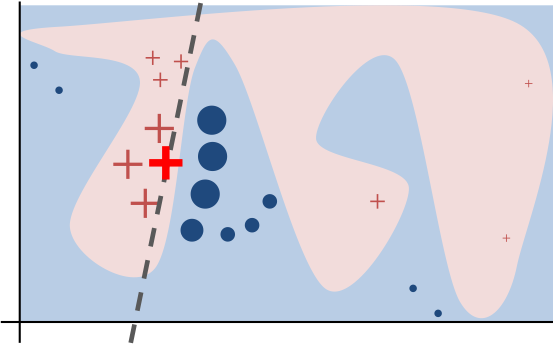
\includegraphics[scale=0.7]{figures/lime.png}
\caption{Toy example to present intuition for LIME. The black-box model's complex decision function $f$ (unknown to LIME) is represented by the blue/pink background, which cannot be approximated well by a linear model. The bold red cross is the instance
being explained. LIME samples instances gets predictions using $f$, and weighs them by the proximity to the instance being explained (represented here by size). The dashed line is the learned explanation that is locally (but not globally) faithful \cite{lime}. 
\label{fig:lime}}
\end{figure} 


\subsubsection{ Shap - SHapley Additive exPlanation }
\label{sec:shap}
To understand the final method of analyzing the feature's importance, an explanation of the shapely value and the coalitional game theory need to be provided. The fowling paragraph was adopted from~\cite{GameTheory}. 

\paragraph{Coalitional game} \mbox{}

The coalitional game is a tuple $<N,v>$, where $N=\{1,2,\ldots, n \}$ is a finite set of $n$ players, $v: 2^{N} \rightarrow \mathcal{R}$ is a characteristic function, that describe worth of each coalition. The solution of the game is to find the operator $\phi(v) = (\phi_{1}, \ldots \phi_n ) \in \mathcal{R}^n$, which assigns to $<N,v>$ vector of payoffs for each coalition participant. To find a fair solution operator $\phi(v)$ needs to fulfill the following axioms: 

\begin{itemize}
\item  $\sum_{i \in N} \phi_{i}(v)= v(N)$, where $v(N)$ is a value of grand coalition consisting of all players. This axiom is called \textit{efficiency axiom}. 
\item if for two players $i$ and $j$ $v(S\cup \{i\}) = v(S \cup \{j\})$ holds for every $S$, where $S \subset N$ and $i,j \notin S$, then $\phi_{i}(v)= \phi_{j}(v)$. This axiom indicates symmetry property. 
 \item The \textit{dummy axiom} says if $v(S\cup \{i\}) =v(S)$ holds for every $S \subset N$ and $i \notin S$, then $\phi_i(S) = 0$, and the player $i$ is a dummy player, who has no influence on the coalition game outcome. 
 \item for any pair of games $v,w: \phi(w+v)= \phi(w)+\phi(v)$. This property is called additivity axiom.   
\end{itemize}

Shapley theorem says, that for a given game $<N,v>$ exists a unique solution $\phi$, which satisfies above axioms, and it is called the Sapley value:
\begin{equation}\label{eq:shapley_value}
    \phi_{i}^{shapley}(v) = \sum_{S \subseteq N, s=|S|} \frac{(n-s-1)!s!}{n!}(v(S\cup \{i\}) - v(S)))
\end{equation}

The proof of the above theorem can be found in the original Shapley's paper \cite{ShapleyProof}. 

To illustrate, let us consider a United Nations Security Council example. The UN council consists of 5 permanent members, namely China, Russia, France, the UK, and the US, with veto power and ten non-permanent members. All permanent members must not veto, and the majority of members need to agree to pass the resolution.  What is the Shapley value for each of the countries? 

To simplify the example let us consider the game $N = \{1,2,3 \}$ . The player $1$ is a permanent member with the veto power, and players $2$ and $3$ are non-permanent members. The value of this game is expressed: $ v( \{1,2 \})= v( \{1,3 \})= v( \{1,2,3\})=1$ and $v(S)=0$ otherwise. 
The Shapley value for this game obtained using formula \ref{eq:shapley_value} is 
$\varphi_{1} = \frac{2}{3},\varphi_{2}= \frac{1}{6}, \varphi_{3 } =  \frac{1}{6} $.  The conclusion is that both players $2$ and $3$ generate some value, so they deserve to get some reward and the player $1$ gets the most of the reward, because it is the most important since no resolution can be made without it. 

\paragraph{Shap method} \mbox{}

To leverage the idea of the Shapley value for the problem of model explanation let assume that the explanation model $g$ defined in the section \ref{sec:lime} is a linear function of a binary variables: 

\begin{equation}
    g(z') = \phi_0 + \sum_{i=1}^{M} \phi_{i}z_i'
\end{equation}
where $z' \in \{ 0, 1\}^{M}$ indicates whether the feature was observed ($z'=1$) or unknown ($z'=0$), and $\phi_i \in \mathcal{R}$ are feature's value.

In order to evaluate the effect of missing features $i$ on the model being explained $f$, it is necessary to define a mapping $h_x$, that each missing binary feature $z'$ maps to the original function. Such a mapping allows calculating the effect $f(h_x(z'))$ of observing or not features. To compute the Shap values, the authors proposed \cite{shap} the following assumption: 

\begin{equation} \label{eq:shap assumtion}
    f(h_x(z')) = \mathbf{E}[f(x)|x_S]
\end{equation}

where S is the set of non-zero indexes in $z'$, and $\mathbf{E}[f(x)|x_S]$ is the expected value of the function $f(x)$ conditioned on a subset $S$ of the input features. Putting together equation \ref{eq:shap assumtion} and \ref{eq:shapley_value} the shap value is calculated using the following formula:

\begin{equation}
        \phi_{i} = \sum_{S \subseteq N} \frac{(M-|S|-1)!|S|!}{M!}(\mathbf{E}[f(x)| S\cup \{i\}] - \mathbf{E}[f(x)|S])
\end{equation}

Figure \ref{fig:shap_exp} visualize the idea of model explanation and feature importance based on a Shap method. 


\begin{figure}[!h]
\centering
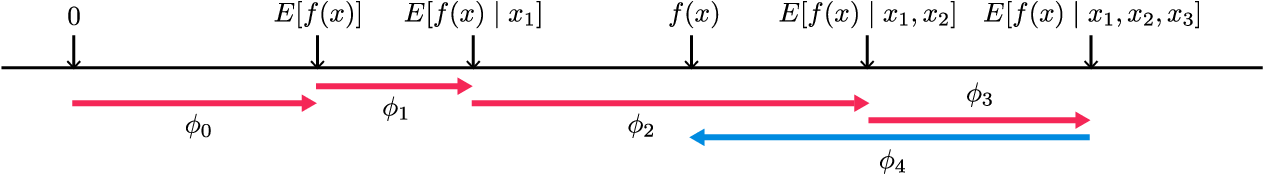
\includegraphics{figures/shap_explanation.png}
\caption{Shap values explain the output of a function $f$ as a sum of the effect $\phi_i$ of each feature being introduced into a conditional expectation \cite{shap2}. 
\label{fig:shap_exp}}
\end{figure} 


\section{bonsai Boosted Decision Tree}
\label{sec:bbdt}
Since the tracking algorithm is a part of the real-time LHCb High-Level Trigger system, both the execution time and memory footprint are important, so using the full continuous classifier is not an option. Instead, a binned BDT (called bonsai BDT or bBDT ) classifier that meets the speed and memory criteria of the HLT is used. This section is dedicated to present the idea of the model's binarization, and the benefits drawback will be discussed. Similar idea was implemented within the LHCb HLT \cite{bbdt}.


The idea is to replace the evaluation of each tree that constitutes the Gradient Boosted Classifier model \footnote{From the technical perspective gradient boosted model is very close to the big array of if-else statements} into an operation that is independent of the model's complexity. The best possible choice for such an operation would be the one that has a constant time computation complexity O(1).  A lookup table \footnote{The lookup table should be implemented as a hash table} is the right candidate. Thus it is a data structure that fulfils the above access time requirement. The remaining problem is how to convert a complex model into the lookup table.  The solution to this problem is data discretization, which is a process of splitting an input space into $k$ bins, and then for each of the combinations of the bins, the model's prediction is calculated, and the obtained value is saved. 

To get a better understanding of how this process works, consider a 2D binary classification problem where "X" and "0" represent two possible classes, which are shown in figure \ref{fig:bbdt_theory}. For simplicity, let the number of bins $k=2$, therefore in order to discretize the models, one needs to calculate four predictions, which is a number of bins times number of features. The outcome of this process is a table presented on the right side of figure \ref{fig:bbdt_theory}. In order to calculate the prediction for a given new instance x (denoted as a red dot), the classifier needs to find corresponding bin indices and extract value from the table. In this example, the prediction is 1. 



\begin{figure}[!h]
\centering
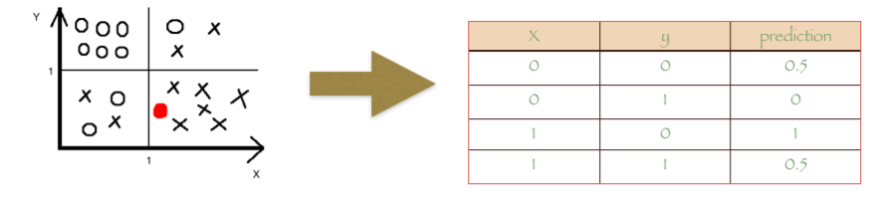
\includegraphics{figures/BBDT_explanation.png}
\caption{bonsai Boosted Decision Tree idea visualization, see text for an explanation
\label{fig:bbdt_theory}}
\end{figure} 